%-------------------------------------------------------------------------
%-------------------------------------------------------------------------
%-------------------------------------------------------------------------

\chapter[Appendix: Design Study]{Design Study Supplemental Material}
\label{app:emu}

%-------------------------------------------------------------------------
%-------------------------------------------------------------------------
%-------------------------------------------------------------------------

This appendix supports \autoref{ch:emu}. 
It contains our original project proposal (Summer 2013) and example research artefacts (Fall 2013 through Summer 2014).

%-------------------------------------------------------------------------
%-------------------------------------------------------------------------

\section{Design Study Proposal}
\label{app:emu:proposal}

%-------------------------------------------------------------------------
%-------------------------------------------------------------------------

\footnote{This research proposal for the design study project was written in Summer 2013, during the first half of the work domain analysis phase.}This project proposal pertains to the domain of large-scale energy management\index{energy management}. 
At a high level, the goal of this project is to improve the process by which professional energy managers\index{energy management} and utility company personnel analyze large amounts of data related to energy consumption. 
This process is often exploratory, meaning that not all analysis questions can be phrased as a directed query or a detailed hypothesis. 
Open-ended exploration can be supported by visualization, which involves a collection of techniques for representing and interacting with large amounts and varying types of data. 
Visualization techniques and tools provides analysts with an overview of the data, as well as an ability to drill down into specific subsets of the data as their analysis questions are refined. 
The application of visualization techniques to the problem of large-scale energy management\index{energy management} will involve implementing and adapting an iterative user-centred design and evaluation\index{evaluation} process. 
The results of this project are expected to be of value to those working in the domain of energy management\index{energy management} as well as visualization practitioners and user experience researchers working in other application domains.

%-------------------------------------------------------------------------
\subsection{Domain Background}
\label{app:emu:proposal-background}
%-------------------------------------------------------------------------

Energy-conscious organizations are seeking ways to better understand energy consumption information beyond their monthly utility invoices; many are interested in identifying ways to conserve energy. 
However, while access to energy consumption data increases, the scale and complexity of the data is also growing; for example, with the emergence of Smart Meter technology it will soon be possible to collect energy consumption data at the level of rooms or individual appliances. 
As this deluge of data continues, effective means\index{task!means} for presenting and analyzing energy consumption data are needed. 
The research community has responded with a number of applications and techniques for providing energy consumption feedback, often referred to as eco-feedback~\cite{Froehlich2010}. 
These predominantly address personal or domestic energy consumption, and includes recent work by \citet{Goodwin2013}, in which visualization is used to assist energy analysts in understanding and modeling domestic energy consumption. 
Eco-feedback displays are also being designed for direct use by home owners, from ambient visual encodings\index{visual encoding} embedded into household displays~\cite{Rodgers2011} to web portals with detailed graphical displays~\cite{Erickson2013}. 
However, little research to date has addressed energy management\index{energy management} for large organizations, such as universities, corporations, governments, or energy providers. 
Consider a university facilities manager who oversees the energy management\index{energy management} of all buildings on a large campus, a corporate facilities manager responsible for multiple properties spanning different geographical regions, or a utility company analyst who has access to energy consumption data for thousands of buildings. 
Pulse Energy\footnote{Pulse Energy has since been acquired by EnerNOC: \url{http://www.enernoc.com/}.} provides a number of commercial energy management\index{energy management} solutions, ranging from detailed summary reports for small business owners to advanced interactive analysis applications for professional energy managers\index{energy management} at larger organizations. 
Some of this feedback already involves visual encodings\index{visual encoding} such as line graphs\index{visual encoding!line graph} and bar charts\index{visual encoding!bar chart}; while useful, these cannot at present support a growing number of analysis questions, nor do they scale the size and heterogeneity of the data collected. 
Pulse Energy is seeking to improve the analysis workflow\index{workflows} of professional energy analysts, which involves the identification of energy consumption patterns, the detection of anomalies, and the prediction of future energy consumption together with measures of confidence. 
This analysis requires an integration of data having varying scale and type, including raw and aggregated energy consumption, detailed weather information, as well as building size, location, operating hours, and occupancy.

%-------------------------------------------------------------------------
\subsection{Information Visualization Background}
\label{app:emu:proposal-infovis-background}
%-------------------------------------------------------------------------

A number of existing visualization techniques may be suitable for representing and interacting with heterogeneous energy consumption data. 
However, the scope of visualization research involves much more than merely implementing known techniques. 
According to Munzner's nested model\index{nested model (Munzner)} for visualization design and validation~\cite{Munzner2009}, visualization research can be considered at four levels. 
The first level involves the characterization of a domain problem; our domain problem, as we currently understand it, is for energy managers\index{energy management} to better understand patterns and variations in energy consumption over time and across multiple buildings, as well as a need for predicting future energy consumption. 
The second level involves the translating this problem into a set of domain-agnostic abstract data types\index{data abstraction} and tasks\index{task!task abstraction}. 
With regards to abstract data\index{data abstraction} types, our current understanding of the problem suggests that we will be faced with largely quantitative multivariate time-oriented data, as well as some spatial data variables. 
With regards to abstract tasks\index{task!task abstraction}, our current understanding of the problem suggests high-level {\tt present}\index{{\tt present}} and {\tt discovery}\index{{\tt discover}} tasks\index{task!high-level tasks}, which in turn involve searching\index{{\tt search}} for values and patterns, as well as {\tt identifying}\index{{\tt identify}}, {\tt comparing}\index{{\tt compare}}, and {\tt summarizing}\index{{\tt summarize}} these results. 
Further analysis of the problem will be required to definitively identify abstract data\index{data abstraction} types and tasks\index{task!task abstraction}, their prevalence, and their relative importance. 
The third level involves the selection of appropriate visual encoding\index{visual encoding} and interaction\index{interaction} design choices that map to these abstract data\index{data abstraction} types and tasks\index{task!task abstraction}; many techniques have been developed for the analysis of time-related data~\cite{Aigner2011}. 
Techniques for representing uncertainty\index{uncertainty} in data~\cite{MacEachren2012} may be of use for the analysis questions pertaining to simulation, anomaly detection, and predictions of future energy consumption. 
We may also leverage visualization design choices for the {\tt filtering}\index{{\tt filter}}, {\tt aggregation}\index{{\tt aggregate}}, {\tt selection}\index{{\tt select}}, {\tt navigation}\index{{\tt navigate}}, {\tt arrangement}\index{{\tt arrange}}, and alteration ({\tt changing}\index{{\tt change}}) of data. 
Finally, the fourth level pertains to the design of algorithms\index{algorithms} that drive the design choices, which is of particular concern to those developing novel visual encoding\index{visual encoding} or interaction\index{interaction} design choices; at this time, it is not apparent that novel design choices will be required for this project. 
At each level, design choices must be evaluated\index{evaluation}, to which there exists a growing repertoire of suitable evaluation\index{evaluation} methods and methodologies~\cite{Lam2012,Meyer2015}. 
Within the visualization research community, projects traversing these four levels are known as design studies. 
The contributions of a design study\index{design studies} paper include the identification of domain-agnostic task\index{task!task abstraction} and data abstractions\index{data abstraction}, a well-reasoned mapping of these abstractions to appropriate design choices, and a critical reflection of design and evaluation\index{evaluation} process, thereby providing guidance to other visualization practitioners working in similar and different application domains.

%-------------------------------------------------------------------------
\subsection{Objectives}
\label{app:emu:proposal-objectives}
%-------------------------------------------------------------------------

The objectives of this project are as follows:

\begin{enumerate}
    \item Identify energy management\index{energy management} tasks and practices, documenting what works well as well as current unmet analysis goals of collaborating energy managers\index{energy management}.
    \item Given (1), derive domain-agnostic data\index{data abstraction} and task abstractions\index{task!task abstraction} and consider appropriate visual encoding\index{visual encoding} and interaction\index{interaction} design choices.
    \item Engage in an iterative participatory design process with collaborating energy managers\index{energy management} and other project stakeholders.
    \item Deploy and evaluate\index{evaluation} resulting designs as a component of the existing Energy Manager\index{Energy Manager} application, determining whether it meets the needs of energy analysts\index{energy management}.
    \item Document and reflect upon the design process and introduce or improve guidelines for visualization practitioners doing similar work in (a) the energy management\index{energy management} domain, (b) in domains with time-oriented data, (c) domains with exploratory analysis tasks, (d) domains with subject-matter experts.
\end{enumerate}

%-------------------------------------------------------------------------
\subsection{Methodology}
\label{app:emu:proposal-methodology}
%-------------------------------------------------------------------------

This project will progress according to the nine-stage visualization design study methodology of \citet{Sedlmair2012}\index{design studies}. 
The first two stages, {\it learn} and {\it winnow}, are already underway; these stages involve meeting with potential collaborators, learning about their unsolved problems, determining whether a shared research question exists, establishing rapport, and identifying logistical barriers to continued collaboration, such as access to people who will use the visualization tool or technique and representative data. 
This research proposal serves as an indication that these preconditions to collaboration have been satisfied. 
The next stage, {\it cast}, involves identifying and developing relationships with the people who will use the tool or technique and other project stakeholders, as well as determining their level of involvement in subsequent stages. 
% These three initial stages are expected to be complete at the outset of the project. 
The project will focus on the core design and evaluation\index{evaluation} stages: {\it discover}, {\it design}, {\it implement}, and {\it deploy}. 
{\it Discover} refers to the process of identifying abstract data types\index{data abstraction} and tasks\index{task!task abstraction}, while {\it design} refers to the process of mapping appropriate visual encoding\index{visual encoding} and interaction\index{interaction} design choices to these data\index{data abstraction} and task\index{task!task abstraction} abstractions, involving iterative and rapid low-fidelity prototyping and evaluation\index{evaluation}; {\it implement} refers to the development and refinement of a high-fidelity interactive prototype, and {\it deploy} releases the finished visualization tool to the people who will use it, in this case as a component of Pulse's Energy Manager\index{Energy Manager} web application. 
The final two stages, {\it reflect}, and {\it write}, are expected to take place as part of an ongoing research collaboration with Pulse Energy; in the months after deployment, {\it reflect} refers to an ongoing critical examination of the design and evaluation\index{evaluation} process, occurring while longitudinal usage of the visualization tool is recorded.
Finally, {\it write} involves identifying and writing about aspects of our design and evaluation\index{evaluation} process which may benefit other visualization practitioners working in other application domains, such as our selection of specific visual encoding\index{visual encoding} and interaction\index{interaction} design choices, or the efficacy of particular evaluation\index{evaluation} methods. 
Sedlmair \etal's article~\cite{Sedlmair2012} also contains 32 design study pitfalls during the stages of the methodology\index{design studies}; these pitfalls include ignoring existing practices that currently work well ({\it discover} phase), failing to sufficiently abstract data\index{data abstraction} and tasks\index{task!task abstraction} ({\it design} phase), employing non-rapid prototyping methods ({\it implement} phase), and failing to conduct an externally valid case study\index{case study}, assuming that a hypothesized usage scenario is sufficient ({\it deploy} phase). 
These pitfalls are unambiguously worded in that they specify ``what not to do'' in a visualization design study\index{design studies}. 
Altogether, the converse of these pitfalls form a design study checklist.

A breadth of design and evaluation\index{evaluation} methods will be adopted at the four core stages of the methodology. 
Many user-centred design and prototyping methods from the \ac{HCI}\index{human-computer interaction (HCI)} literature~\cite{Dix2004} are appropriate for the design of visualization tools. 
For instance, in the {\it discover} phase, contextual inquiries~\cite{Holtzblatt1993}\index{evaluation!contextual inquiry}, semi-structured interviews, and artefact analysis are useful for understanding the domain context surrounding existing workflows\index{workflows}. 
In the {\it design} and {\it implement} phases, cognitive walkthroughs\index{evaluation!cognitive walkthrough} and think-aloud evaluations~\cite{Dix2004}\index{evaluation!think-aloud evaluation} are useful for identifying usability problems with designs generated during iterative cycles of rapid prototyping. 
In the {\it deploy} phase, follow-up interviews, feature usage statistics extracted from interaction log\index{interaction!interaction logs} files, and artefact analysis help to determine the efficacy of the deployed application.

However, some methods must be adapted to suit the unique aspects of visualization design, particularly during the {\it design} phase. 
\citet{Lloyd2011} stress the importance of using real data in early prototypes, thereby necessitating that prototypes address large-scale datasets and interactive transformations of the data. 
For this reason, traditional paper prototypes are often insufficient for communicating design ideas. 
This leads to a pitfall in which stakeholders exposed to these higher-fidelity interactive prototypes react in a different manner than they would have with low-fidelity paper prototypes. 
For this reason, early prototypes should be presented as ``sketches''~\cite{Wood2012}\index{data sketch}. 
During the {\it design} and {\it implement} stages we will draw from our knowledge of visual encoding\index{visual encoding} and interaction\index{interaction} design choices, particularly those used for time-oriented data~\cite{Aigner2011}\index{time-oriented data}.

Regarding evaluation\index{evaluation}, we will consider the following methods during the {\it design} and {\it implement} stages~\cite{Lam2012}, subject to logistical and timeline constraints~\cite{Sedlmair2011}. 
Heuristic evaluation~\cite{Nielsen1990}\index{evaluation!heuristic evaluation}, individual and group usability interviews, chauffeured demos~\cite{Lloyd2011}\index{chauffeured demos}, and design critiques are among these methods. 
At the {\it deploy} stage, we will use longitudinal evaluation\index{evaluation} methods, often associated with multidimensional in-depth long-term case studies~\cite{Shneiderman2006}\index{case study}, which include interaction log\index{interaction!interaction logs} file analysis~\cite{Pohl2010}, insight diaries~\cite{North2011}\index{evaluation!insight-based evaluation}\index{insight}, and multiple follow-up interviews with project stakeholders. 
We do not foresee the use of formal laboratory-based experiments to evaluate\index{evaluation} our design, unless our design includes novel or untested visual encoding\index{visual encoding} or interaction\index{interaction} design choices.

In design studies\index{design studies}, it is common practice to work closely with stakeholders, those being experts in their domain and sources of invaluable insight\index{insight}. 
These people are considered to be collaborators in a research and design process; they are not considered to be research subjects. 
Nevertheless, should a need arise to elicit feedback from people beyond this core group of collaborators, we may resort to surveys and/or field interviews. 
These methods have been approved by an existing research ethics application (UBC Behavioural Research Ethics Board certificate number H10-03336: “Human Factors in Information Visualization”), and we will file a revision if deemed necessary.

%-------------------------------------------------------------------------
\subsection{Desired Outcome}
\label{app:emu:proposal-outcome}
%-------------------------------------------------------------------------

A desirable outcome of this project is the design of visual encodings\index{visual encoding} and interactions\index{interaction} to support the analysis of large-scale energy consumption data, designs which can be embedded into Pulse Energy's Energy Manager\index{Energy Manager} application. 
This application is widely used by a diverse set of energy managers\index{energy management} and analysts at universities or large distributed organizations, including utility companies. 
It is not intended for the analysis of domestic energy consumption. 
It is our intent that our designs improve energy analysts' understanding of energy consumption, allowing them to make more informed predictions regarding future energy consumption. 
By appealing to these people, Pulse Energy will gain a competitive advantage and is likely to increase adoption\index{adoption} of their services.

%-------------------------------------------------------------------------
\subsection{Milestones}
\label{app:emu:proposal-milestones}
%-------------------------------------------------------------------------

The following milestones are grouped by design study methodology~\cite{Sedlmair2012} phases\index{design studies} (underlined).

\bstart{July 2013 -- October 2013 / early \underline{discover} phase}

\begin{itemize}
    \item Data collection (part-time); site visits and contextual inquiries\index{evaluation!contextual inquiry} with energy analyst collaborators.
\end{itemize}

\bstart{November 2013 / late \underline{discover} phase}

\begin{itemize}
    \item 13.10.28 -– 13.11.01: Wrapping up data collection (site visits and contextual inquiries\index{evaluation!contextual inquiry} with collaborators and stakeholders, begun in July 2013).
    \item 13.11.04 -– 13.11.08: Contextual inquiry\index{evaluation!contextual inquiry} data analysis.
    \item 13.11.11 -– 13.11.15: Participatory ideation and requirements gathering workshop; Remembrance Day holiday (11 / 11).
    \item 13.11.18 -– 13.11.22: Workshop data analysis.
\end{itemize}

\bstart{November -- December 2013 / \underline{design} phase}

\begin{itemize}
    \item 13.11.25 -– 13.11.29: Early design mockups, rapid paper prototyping and internal evaluation\index{evaluation}.
    \item 13.12.02 -– 13.12.06: Rapid {\it sketchy} interactive prototyping and evaluation\index{evaluation}.
    \item 13.12.09 -– 13.12.13: Continued rapid sketchy interactive prototyping and evaluation\index{evaluation}.
    \item 13.12.16 -– 13.12.20: In-house design critiques and heuristic evaluation\index{evaluation}; evaluation\index{evaluation} of sketchy prototypes with representative energy analysts.
\end{itemize}

\bstart{December -- January 2013 / \underline{implement} phase}

\begin{itemize}
    \item 13.12.23 -- 13.12.27: Commitment to particular design; high-fidelity prototype development; Christmas Day holiday (12 / 25).
    \item 13.12.30 -- 13.01.03: High-fidelity prototype development; New Year’s Day holiday (01 / 01).
    \item 14.01.06 -– 14.01.10: Continued high-fidelity prototype development and integration.
    \item 14.01.13 –- 14.01.17: Continued high-fidelity prototype development, integration and in- house evaluation\index{evaluation}.
    \item 14.01.20 –- 14.01.24: Continued high-fidelity prototype development, integration and in-house evaluation\index{evaluation}.
\end{itemize}

\bstart{January -- February 2014 / early \underline{deploy} phase}

\begin{itemize}
    \item 14.01.27 -– 14.01.31: Evaluation\index{evaluation} of integrated prototype with representative energy analysts, tweaking and preparation for deployment.
    \item 14.02.03 -– 14.02.07: Evaluation\index{evaluation} of integrated prototype with representative energy analysts, tweaking and preparation for deployment.
    \item 14.02.10 -– 14.02.14: Deployment of integrated prototype and recruitment of energy analysts for longitudinal study.
    \item 14.02.17 -– 14.02.21: Monitoring of usage data, evaluation\index{evaluation} of deployed prototype begins.
    \item 14.02.24 -- 14.02.28: Follow-up interviews and post-deployment usage data analysis.
\end{itemize}

\bstart{March 2014 -– Spring 2014 / late \underline{deploy} phase, \underline{reflect} and \underline{write} phases}

\begin{itemize}
    \item Continued longitudinal evaluation\index{evaluation} and analysis of deployed prototype, critical reflection, and preparation of a manuscript for submission to a conference or journal.
\end{itemize}

%-------------------------------------------------------------------------
%-------------------------------------------------------------------------

\section{Example Research Artefacts}
\label{app:emu:examples}

%-------------------------------------------------------------------------
%-------------------------------------------------------------------------

The following figures (\ref{app:emu:fig:slide-decks}--\ref{app:emu:fig:storyboards}) and \autoref{app:emu:tab:tasks} are example research artefacts from our design process described in \autoref{emu:methodology}, including examples slides from the eleven slide decks (302 slides in total) generated over the course of this project. 
Slides that attribute individual energy analysts or depict real portfolio data have been sanitized.

%-|-|-|-|-|-|-|-|-|-|-|-|-|-|-|-|-|-|-|-|-|-|-|-|-|-|-|-|-|-|-|-|-|-|-|-|-

\begin{figure}
	\centering
	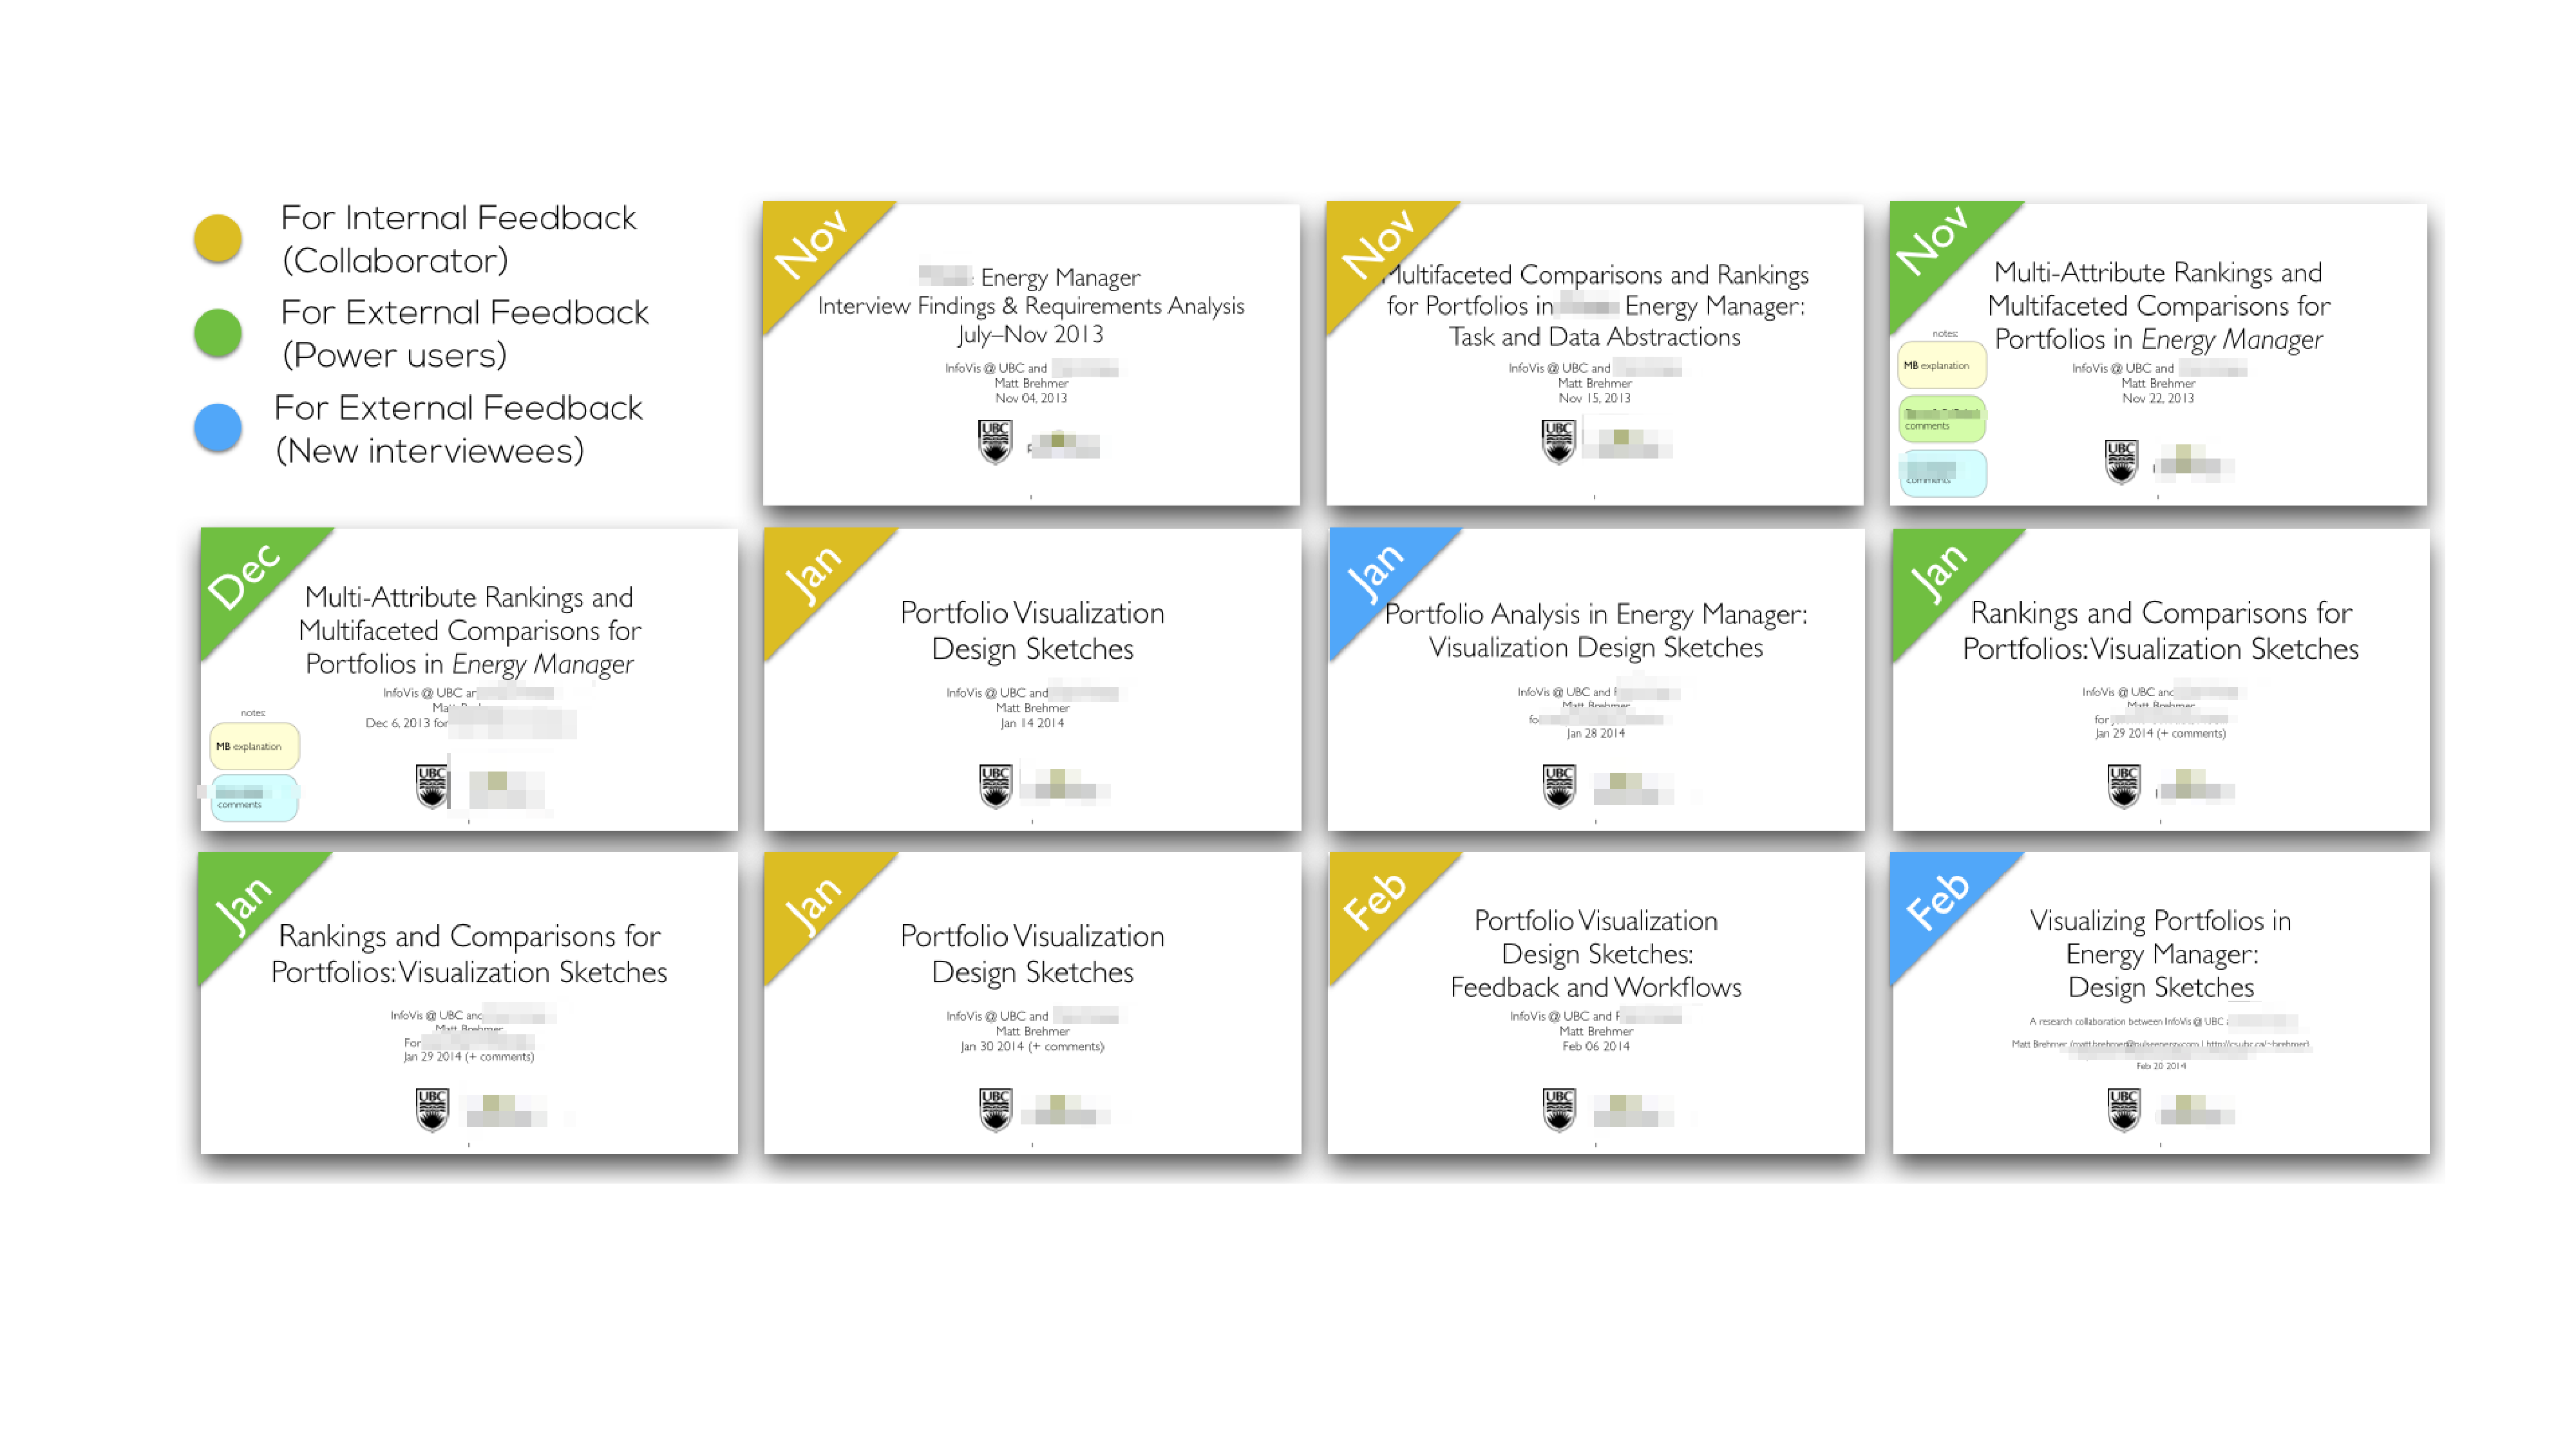
\includegraphics[width=\textwidth]{figures/s-emu-02.pdf}
	\caption
	[
	    Eleven slide decks created between Nov 2013 and February 2014.
	]
	{
    	Eleven slide decks (302 slides in total) created between Nov 2013 and February 2014. Slide decks were iteratively refined research artefacts used to document the research and design process.
	}
	\centering
	\label{app:emu:fig:slide-decks}
\end{figure}

%-|-|-|-|-|-|-|-|-|-|-|-|-|-|-|-|-|-|-|-|-|-|-|-|-|-|-|-|-|-|-|-|-|-|-|-|-

%-|-|-|-|-|-|-|-|-|-|-|-|-|-|-|-|-|-|-|-|-|-|-|-|-|-|-|-|-|-|-|-|-|-|-|-|-

\begin{figure}
	\centering
	\fbox{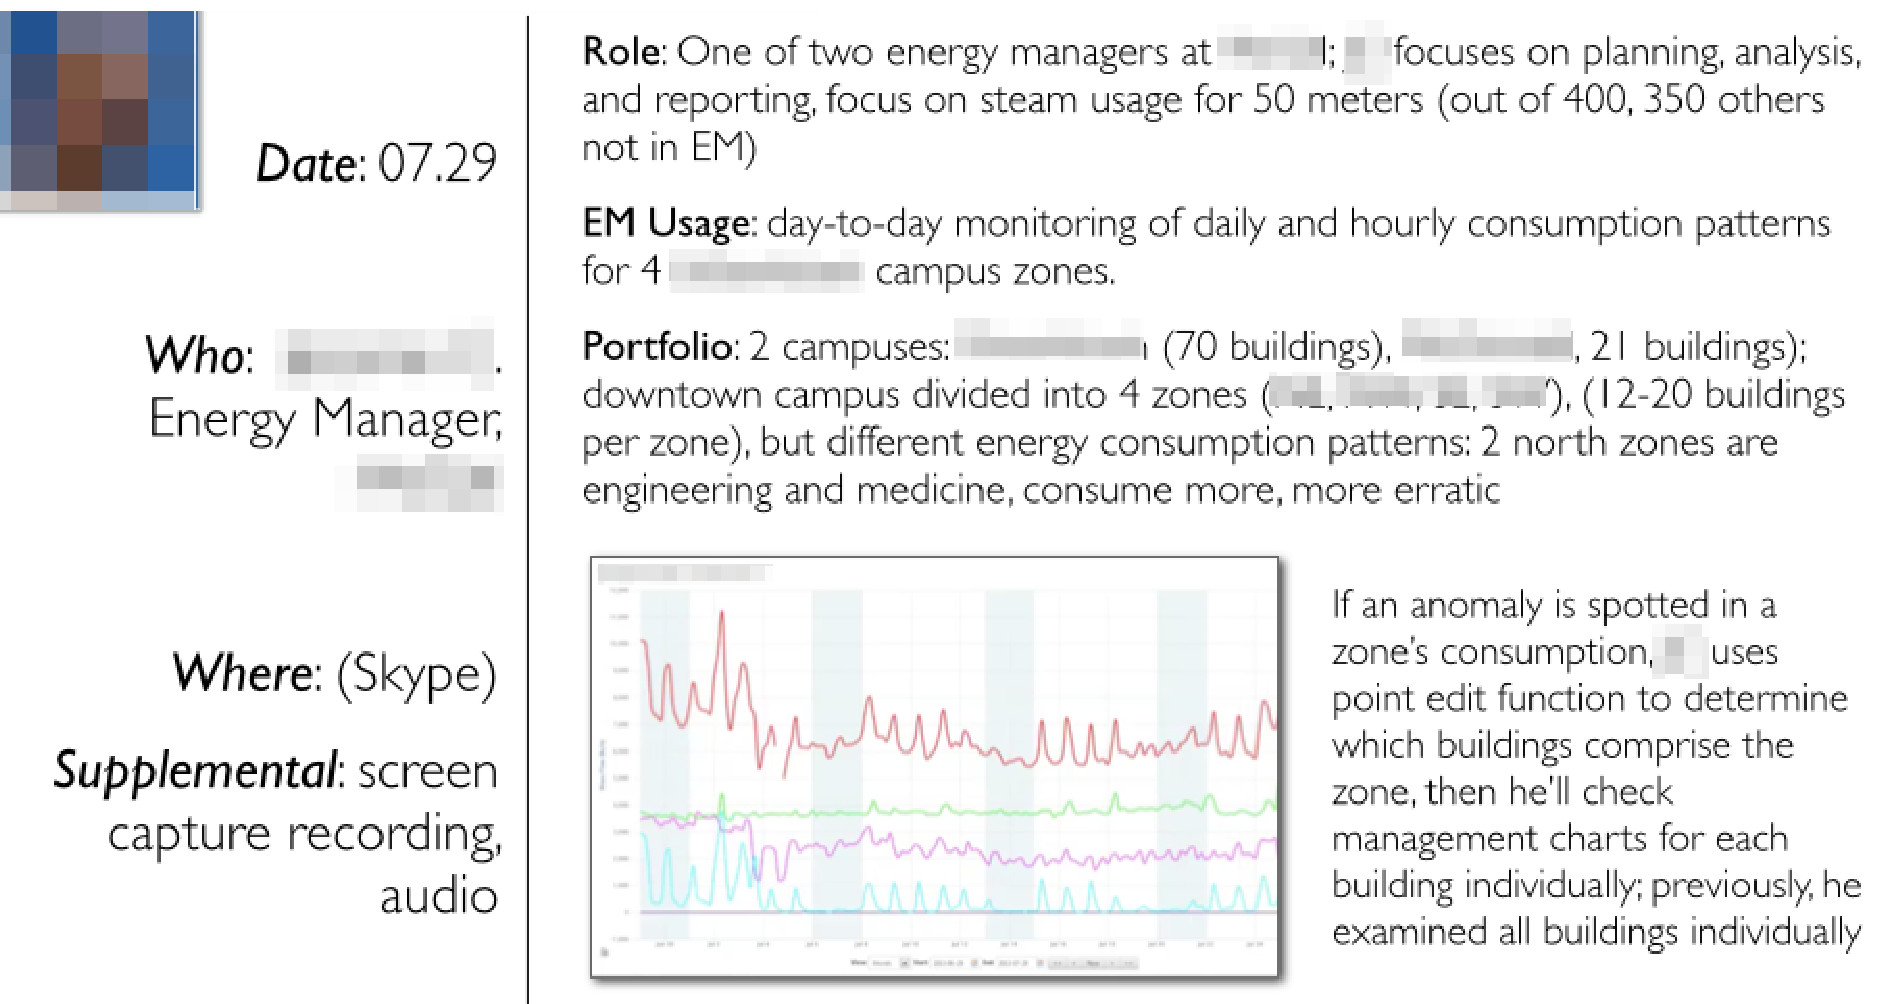
\includegraphics[width=0.975\textwidth]{figures/s-emu-03.pdf}}
	\caption
	[
	    Partial summary of findings from initial interviews with energy analysts.
	]
	{
    	Partial summary of findings from initial interviews with energy analysts (July -- November 2013).  
	}
	\centering
	\label{app:emu:fig:interview-summaries}
\end{figure}

%-|-|-|-|-|-|-|-|-|-|-|-|-|-|-|-|-|-|-|-|-|-|-|-|-|-|-|-|-|-|-|-|-|-|-|-|-

%-|-|-|-|-|-|-|-|-|-|-|-|-|-|-|-|-|-|-|-|-|-|-|-|-|-|-|-|-|-|-|-|-|-|-|-|-

\begin{figure}
	\centering
	\fbox{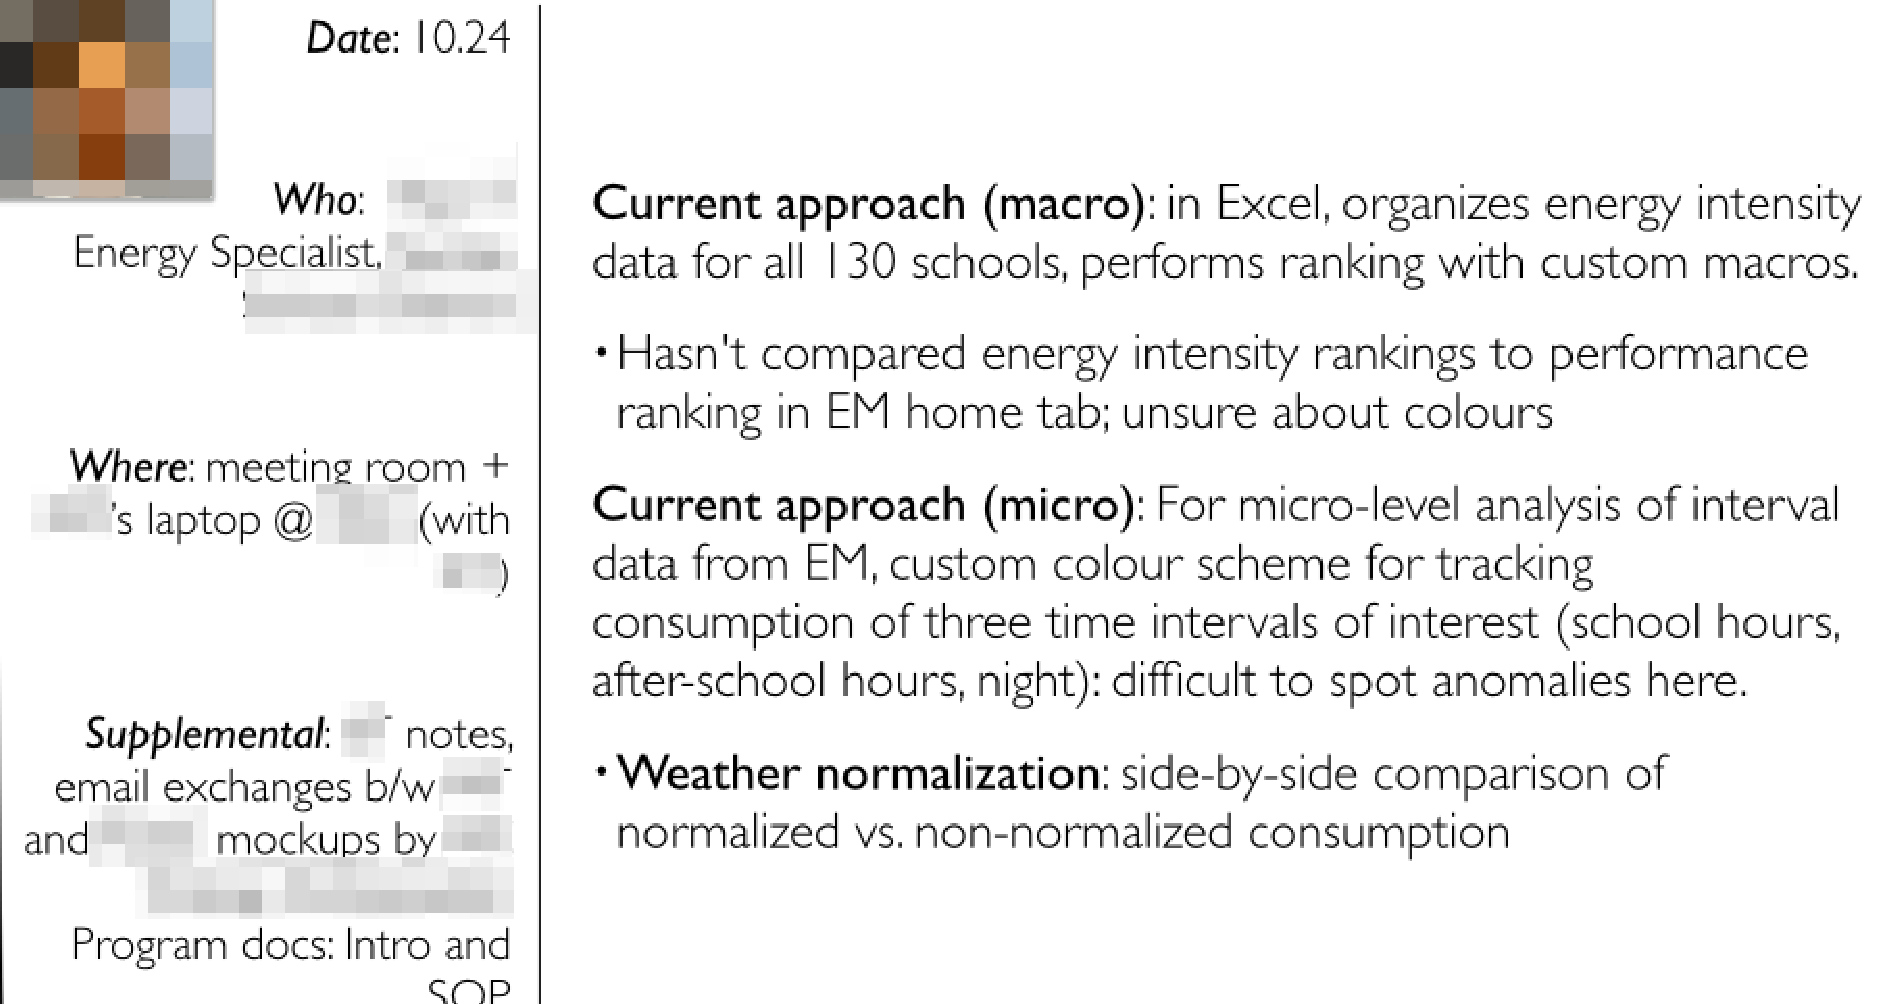
\includegraphics[width=0.975\textwidth]{figures/s-emu-03b.pdf}}
	\caption
	[
	    Partial summary of findings from initial interviews with energy analysts (continued).
	]
	{
    	Partial summary of findings from initial interviews with energy analysts (continued) (July -- November 2013).  
	}
	\centering
	\label{app:emu:fig:interview-summaries-2}
\end{figure}

%-|-|-|-|-|-|-|-|-|-|-|-|-|-|-|-|-|-|-|-|-|-|-|-|-|-|-|-|-|-|-|-|-|-|-|-|-

%-|-|-|-|-|-|-|-|-|-|-|-|-|-|-|-|-|-|-|-|-|-|-|-|-|-|-|-|-|-|-|-|-|-|-|-|-

\begin{table}
	\centering
	\fbox{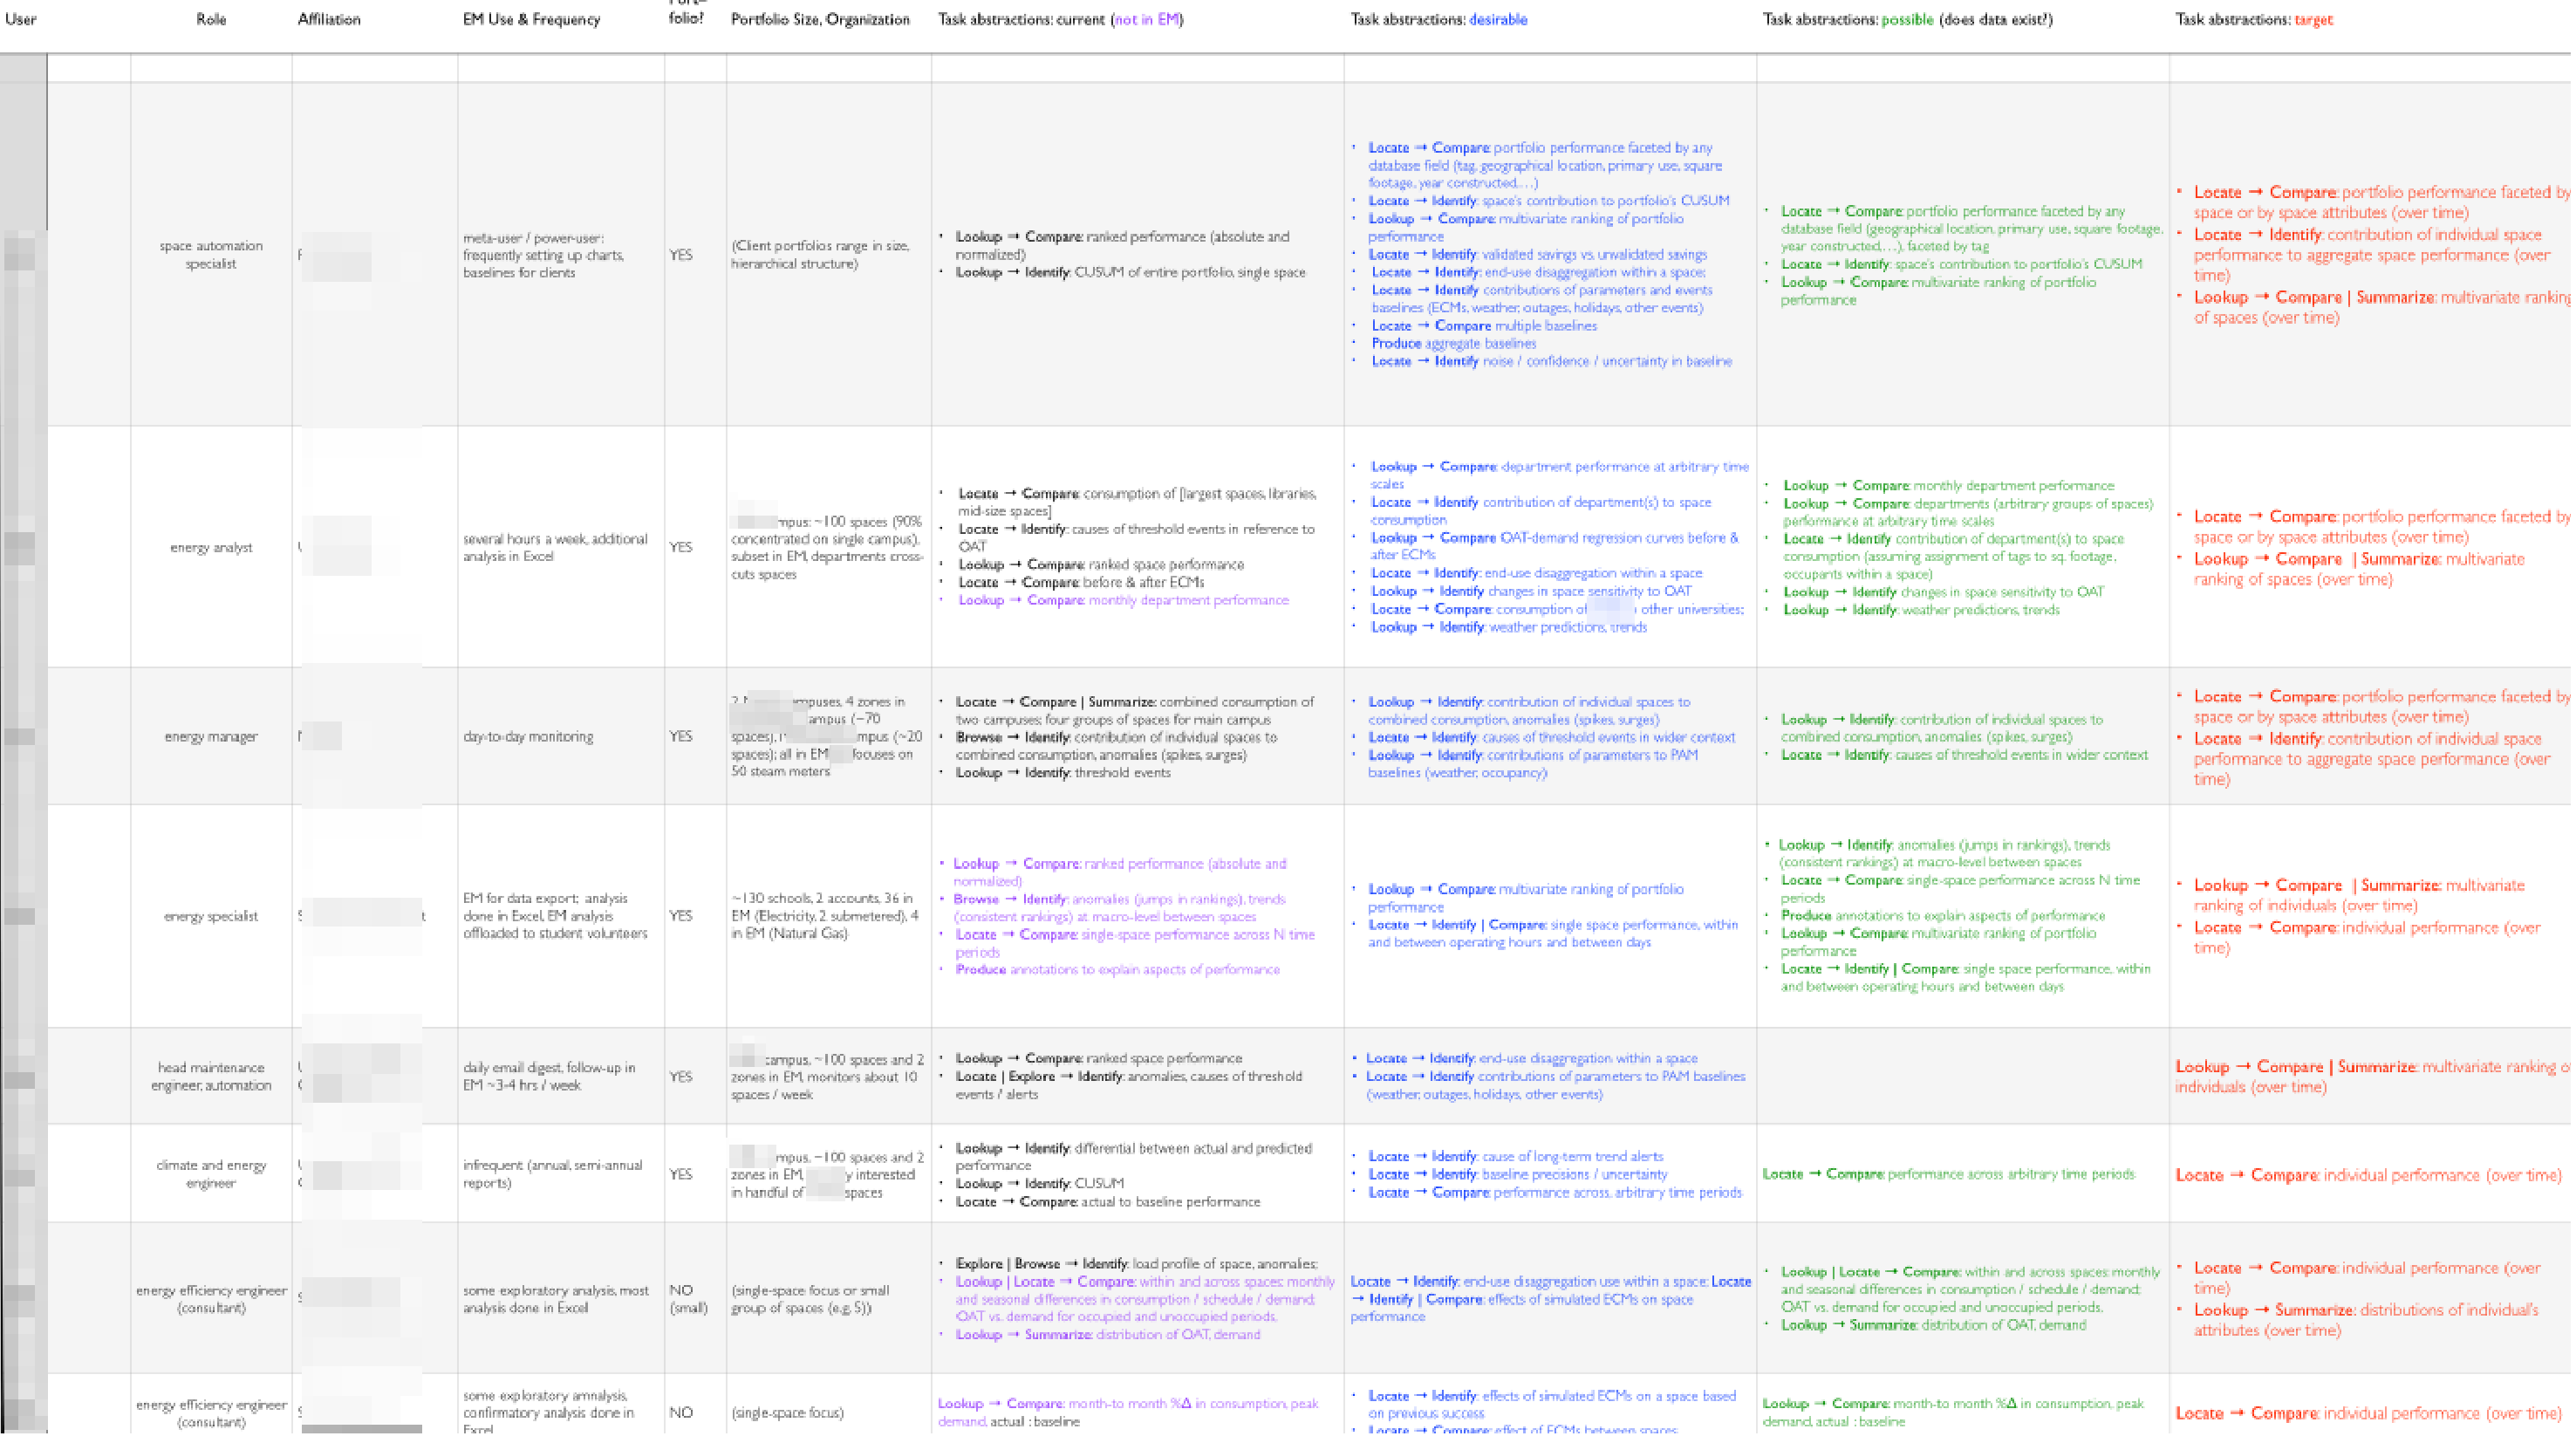
\includegraphics[width=0.975\textwidth]{figures/s-emu-04.pdf}}
	\caption
	[
	    Characterizing energy analyst’s activities as abstract tasks.
	]
	{
    	Characterizing energy analyst's activities as abstract tasks according to our typology proposed in \autoref{ch:typology} (November 2013).  
	}
	\centering
	\label{app:emu:tab:tasks}
\end{table}

%-|-|-|-|-|-|-|-|-|-|-|-|-|-|-|-|-|-|-|-|-|-|-|-|-|-|-|-|-|-|-|-|-|-|-|-|-

%-|-|-|-|-|-|-|-|-|-|-|-|-|-|-|-|-|-|-|-|-|-|-|-|-|-|-|-|-|-|-|-|-|-|-|-|-

\begin{figure}
	\centering
	\fbox{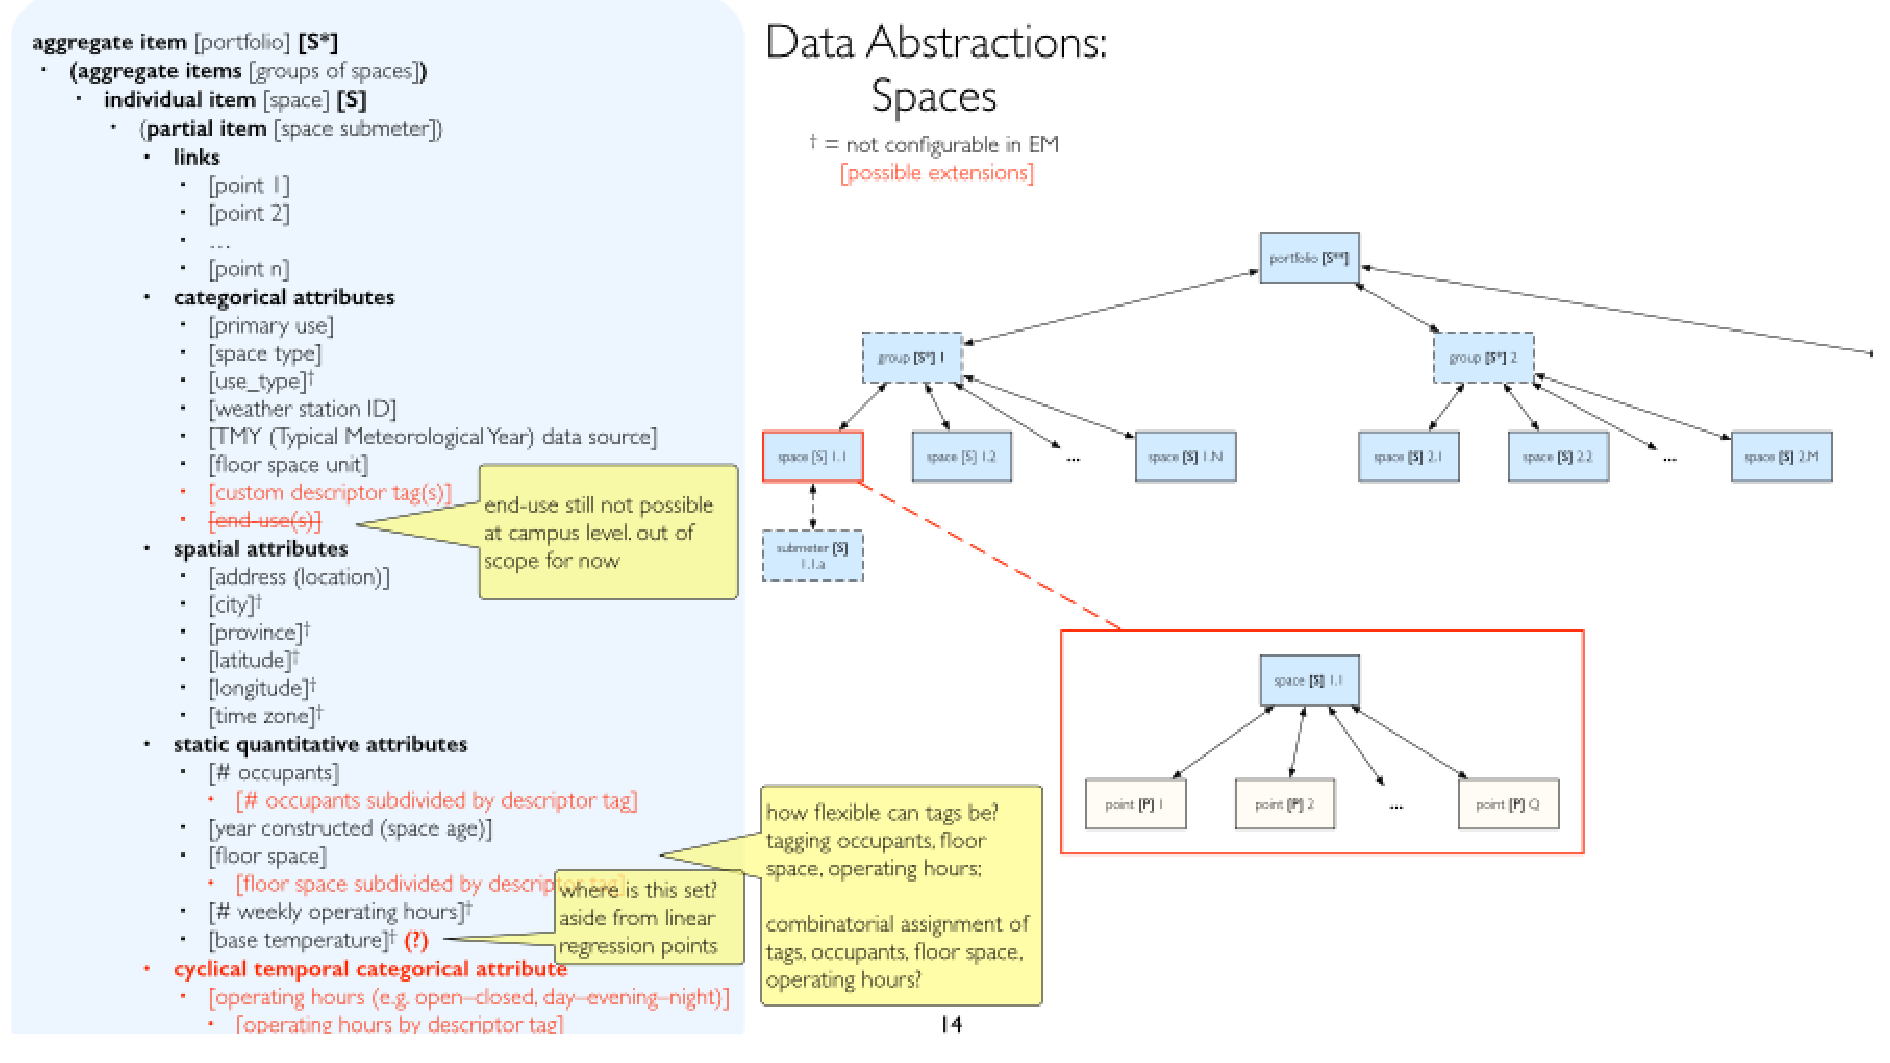
\includegraphics[width=0.975\textwidth]{figures/s-emu-05.pdf}}
	\caption
	[
	    Partial characterization of data abstractions relevant to energy analysts' activities.
	]
	{
    	Partial characterization of data abstractions relevant to energy analysts' activities (November 2013).  
	}
	\centering
	\label{app:emu:fig:data}
\end{figure}

%-|-|-|-|-|-|-|-|-|-|-|-|-|-|-|-|-|-|-|-|-|-|-|-|-|-|-|-|-|-|-|-|-|-|-|-|-

%-|-|-|-|-|-|-|-|-|-|-|-|-|-|-|-|-|-|-|-|-|-|-|-|-|-|-|-|-|-|-|-|-|-|-|-|-

\begin{figure}
	\centering
	\fbox{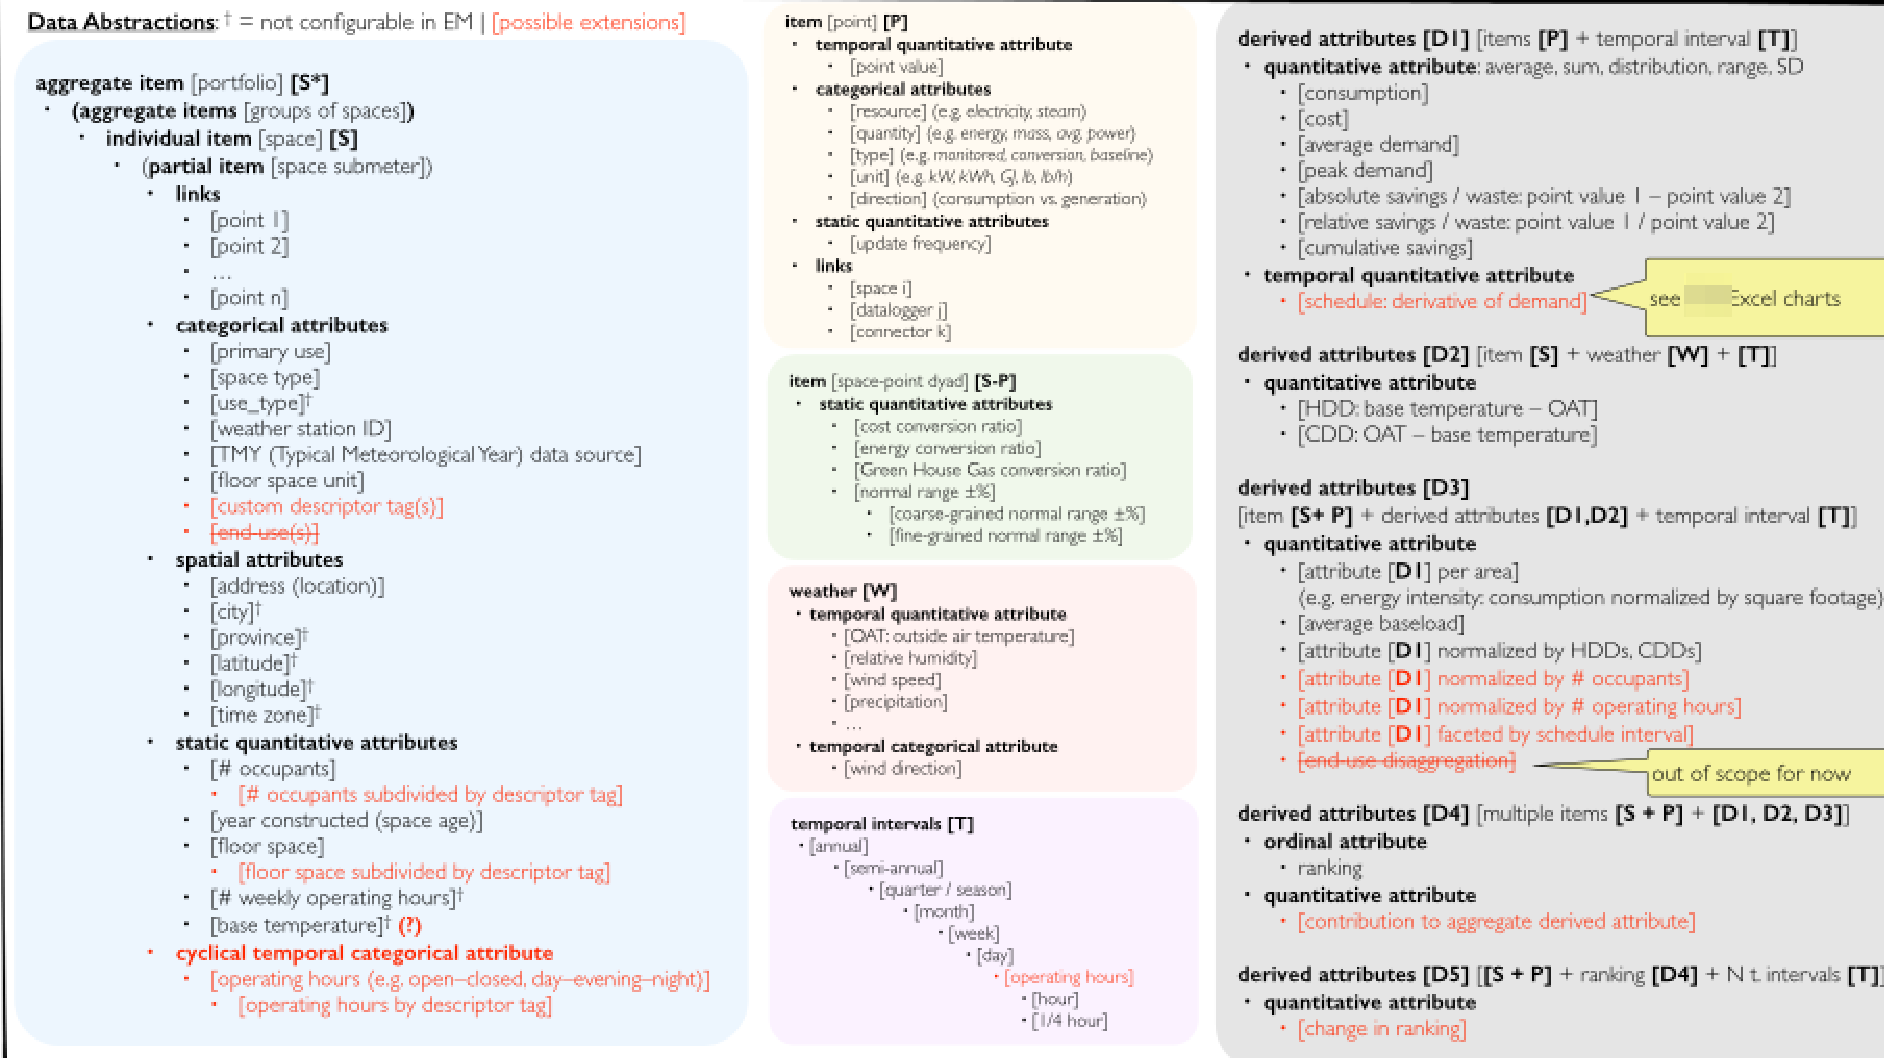
\includegraphics[width=0.975\textwidth]{figures/s-emu-05b.pdf}}
	\caption
	[
	    Partial characterization of data abstractions relevant to energy analysts' activities (continued).
	]
	{
    	Partial characterization of data abstractions relevant to energy analysts' activities (continued) (November 2013).  
	}
	\centering
	\label{app:emu:fig:data-2}
\end{figure}

%-|-|-|-|-|-|-|-|-|-|-|-|-|-|-|-|-|-|-|-|-|-|-|-|-|-|-|-|-|-|-|-|-|-|-|-|-

%-|-|-|-|-|-|-|-|-|-|-|-|-|-|-|-|-|-|-|-|-|-|-|-|-|-|-|-|-|-|-|-|-|-|-|-|-

\begin{figure}
	\centering
	\fbox{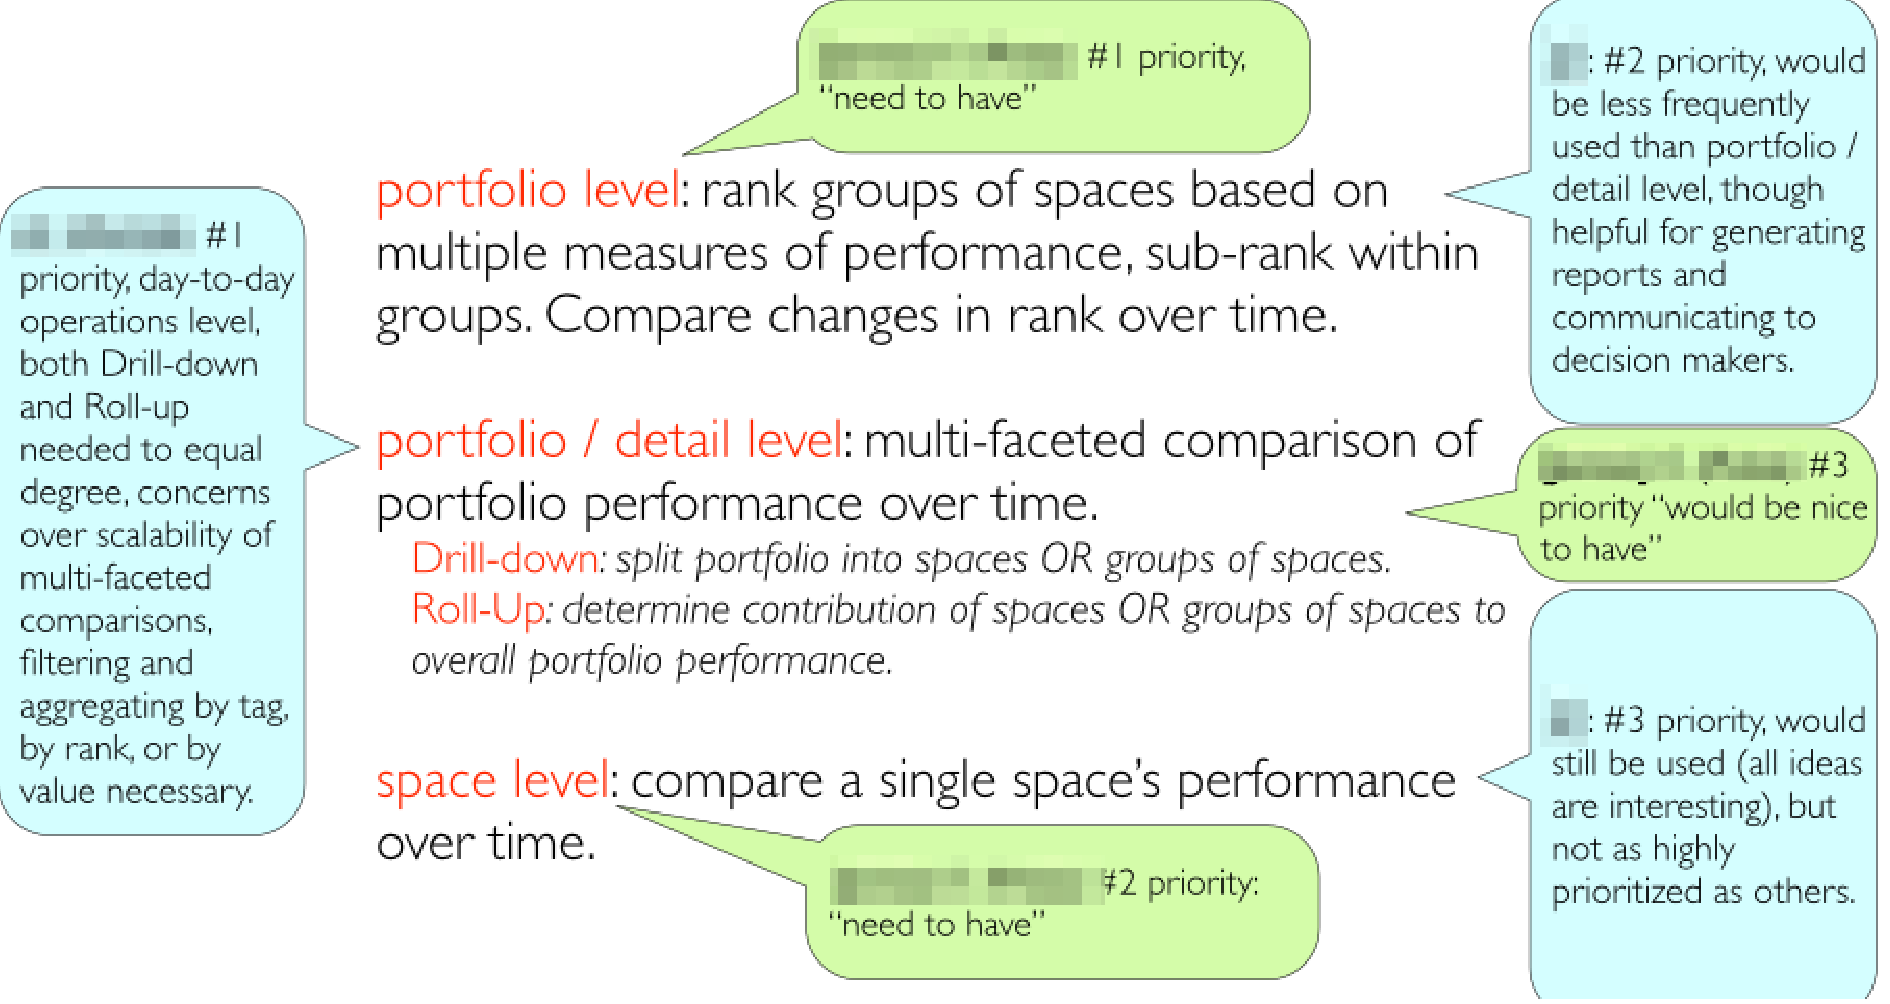
\includegraphics[width=0.975\textwidth]{figures/s-emu-06.pdf}}
	\caption
	[
	    Verifying the task and data abstractions with power user energy analysts.
	]
	{
    	Verifying the task and data abstractions with power user energy analysts: a summary of tasks. (November -- December 2013).  
	}
	\centering
	\label{app:emu:fig:verify}
\end{figure}

%-|-|-|-|-|-|-|-|-|-|-|-|-|-|-|-|-|-|-|-|-|-|-|-|-|-|-|-|-|-|-|-|-|-|-|-|-

%-|-|-|-|-|-|-|-|-|-|-|-|-|-|-|-|-|-|-|-|-|-|-|-|-|-|-|-|-|-|-|-|-|-|-|-|-

\begin{figure}
	\centering
	\fbox{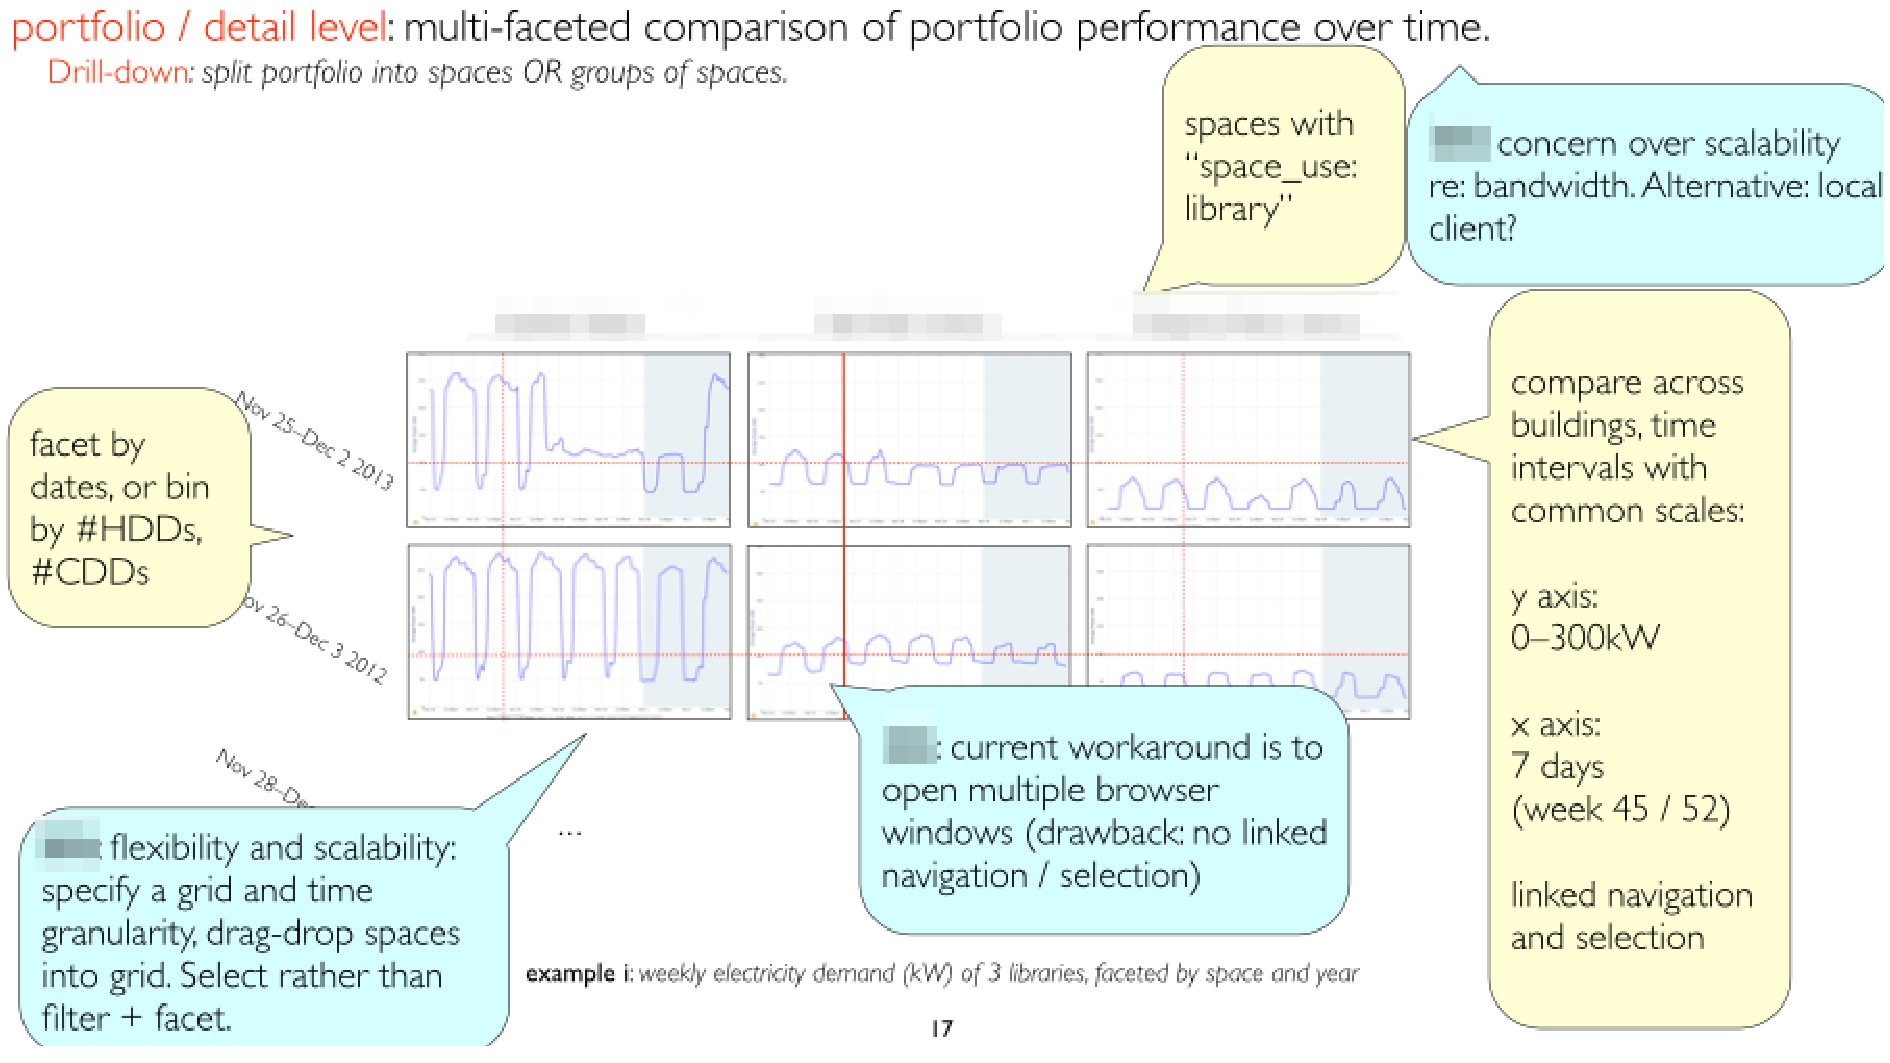
\includegraphics[width=0.975\textwidth]{figures/s-emu-06b.pdf}}
	\caption
	[
	    Verifying the task and data abstractions with power user energy analysts (continued).
	]
	{
    	Verifying the task and data abstractions with power user energy analysts (continued): a mockup of a faceted line graph (November -- December 2013).  
	}
	\centering
	\label{app:emu:fig:verify-2}
\end{figure}

%-|-|-|-|-|-|-|-|-|-|-|-|-|-|-|-|-|-|-|-|-|-|-|-|-|-|-|-|-|-|-|-|-|-|-|-|-

%-|-|-|-|-|-|-|-|-|-|-|-|-|-|-|-|-|-|-|-|-|-|-|-|-|-|-|-|-|-|-|-|-|-|-|-|-

\begin{figure}
	\centering
	\fbox{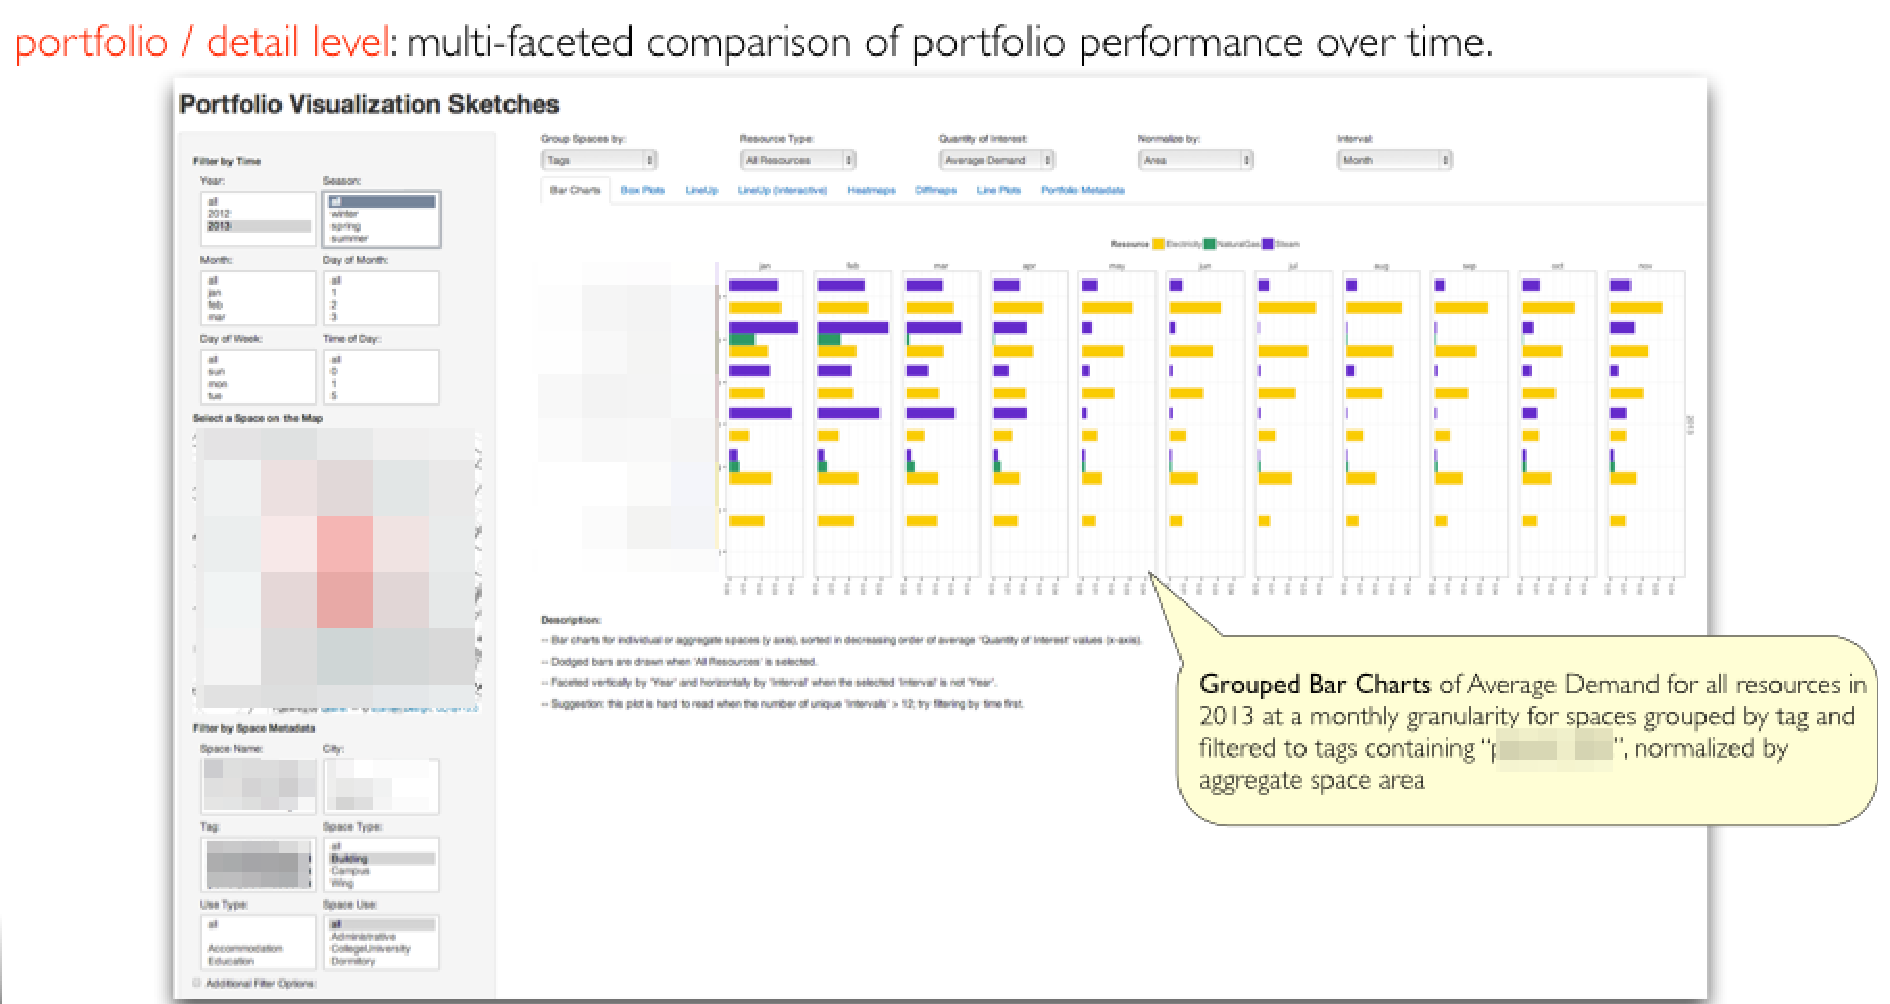
\includegraphics[width=0.975\textwidth]{figures/s-emu-07.pdf}}
	\caption
	[
	    Initial data sketches produced within the sandbox environment.
	]
	{
    	Initial data sketches produced within the sandbox environment: faceted bar charts (January 2014). 
	}
	\centering
	\label{app:emu:fig:initial-sketches}
\end{figure}

%-|-|-|-|-|-|-|-|-|-|-|-|-|-|-|-|-|-|-|-|-|-|-|-|-|-|-|-|-|-|-|-|-|-|-|-|-

%-|-|-|-|-|-|-|-|-|-|-|-|-|-|-|-|-|-|-|-|-|-|-|-|-|-|-|-|-|-|-|-|-|-|-|-|-

\begin{figure}
	\centering
	\fbox{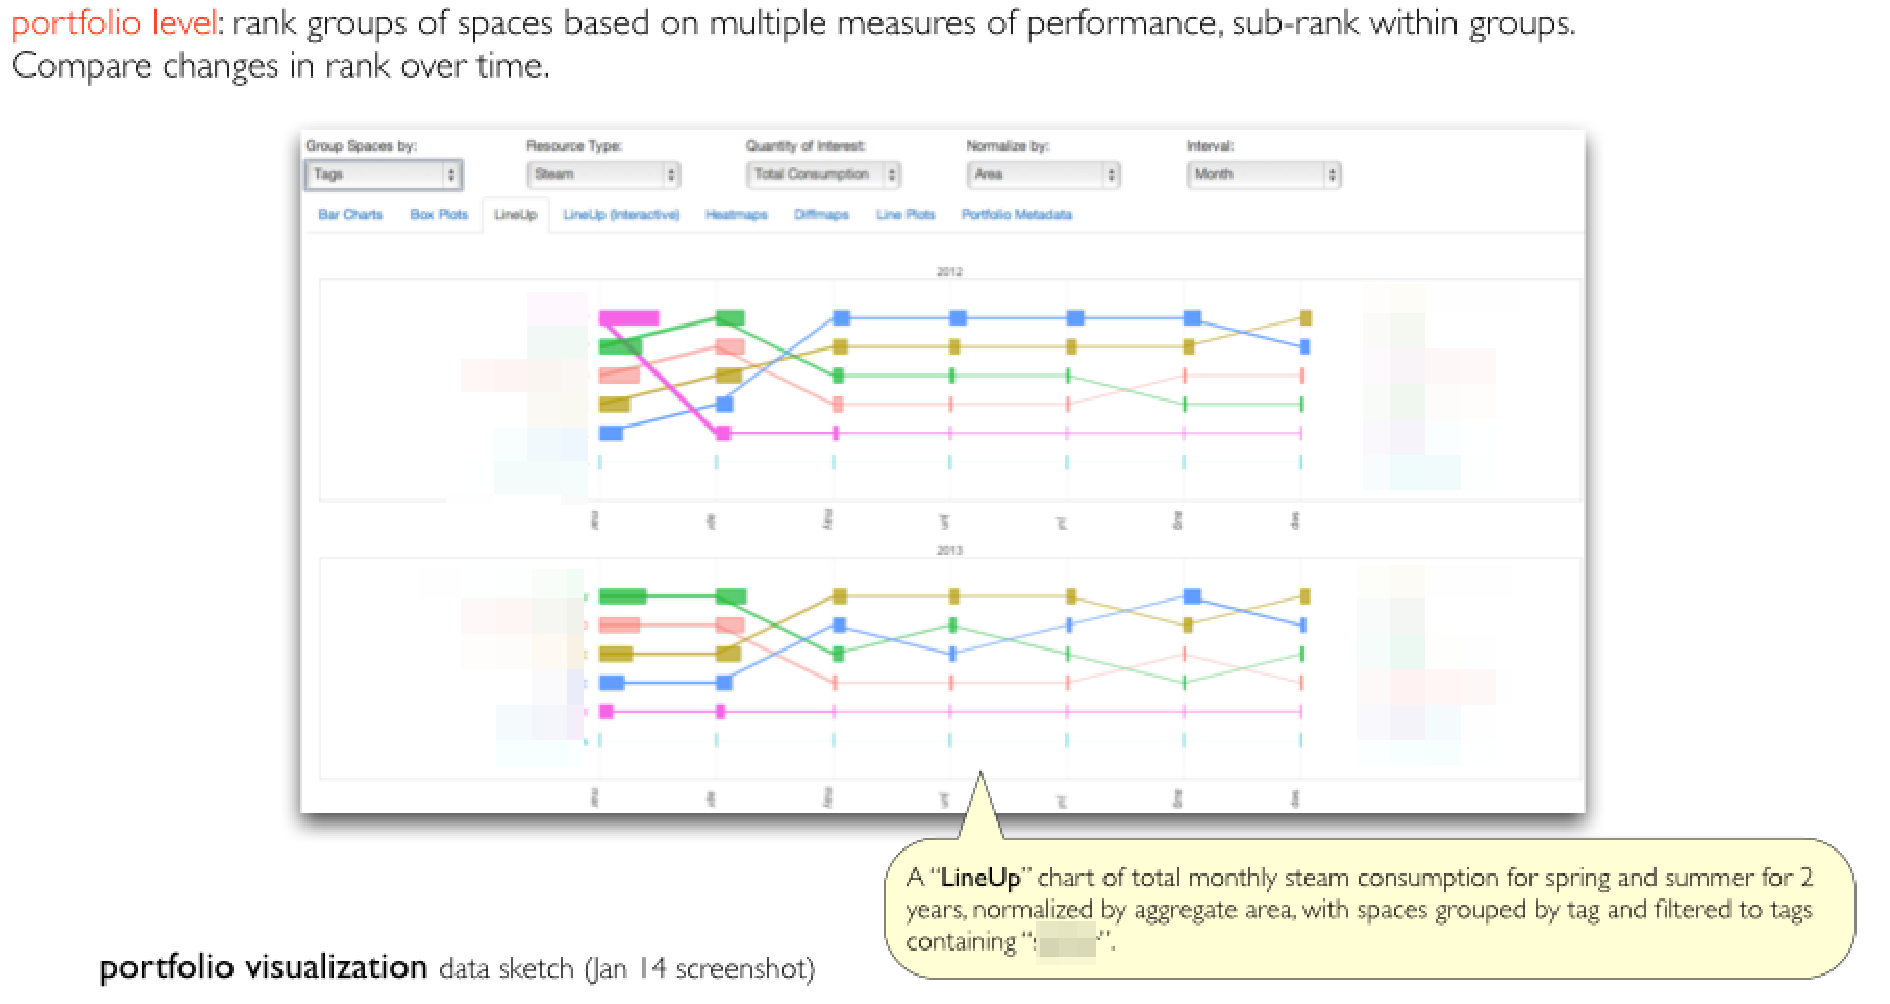
\includegraphics[width=0.975\textwidth]{figures/s-emu-07b.pdf}}
	\caption
	[
	    Initial data sketches produced within the sandbox environment (continued).
	]
	{
    	Initial data sketches produced within the sandbox environment (continued): an early version of the bar + bump plot (January 2014). 
	}
	\centering
	\label{app:emu:fig:initial-sketches-2}
\end{figure}

%-|-|-|-|-|-|-|-|-|-|-|-|-|-|-|-|-|-|-|-|-|-|-|-|-|-|-|-|-|-|-|-|-|-|-|-|-

%-|-|-|-|-|-|-|-|-|-|-|-|-|-|-|-|-|-|-|-|-|-|-|-|-|-|-|-|-|-|-|-|-|-|-|-|-

\begin{figure}
	\centering
	\fbox{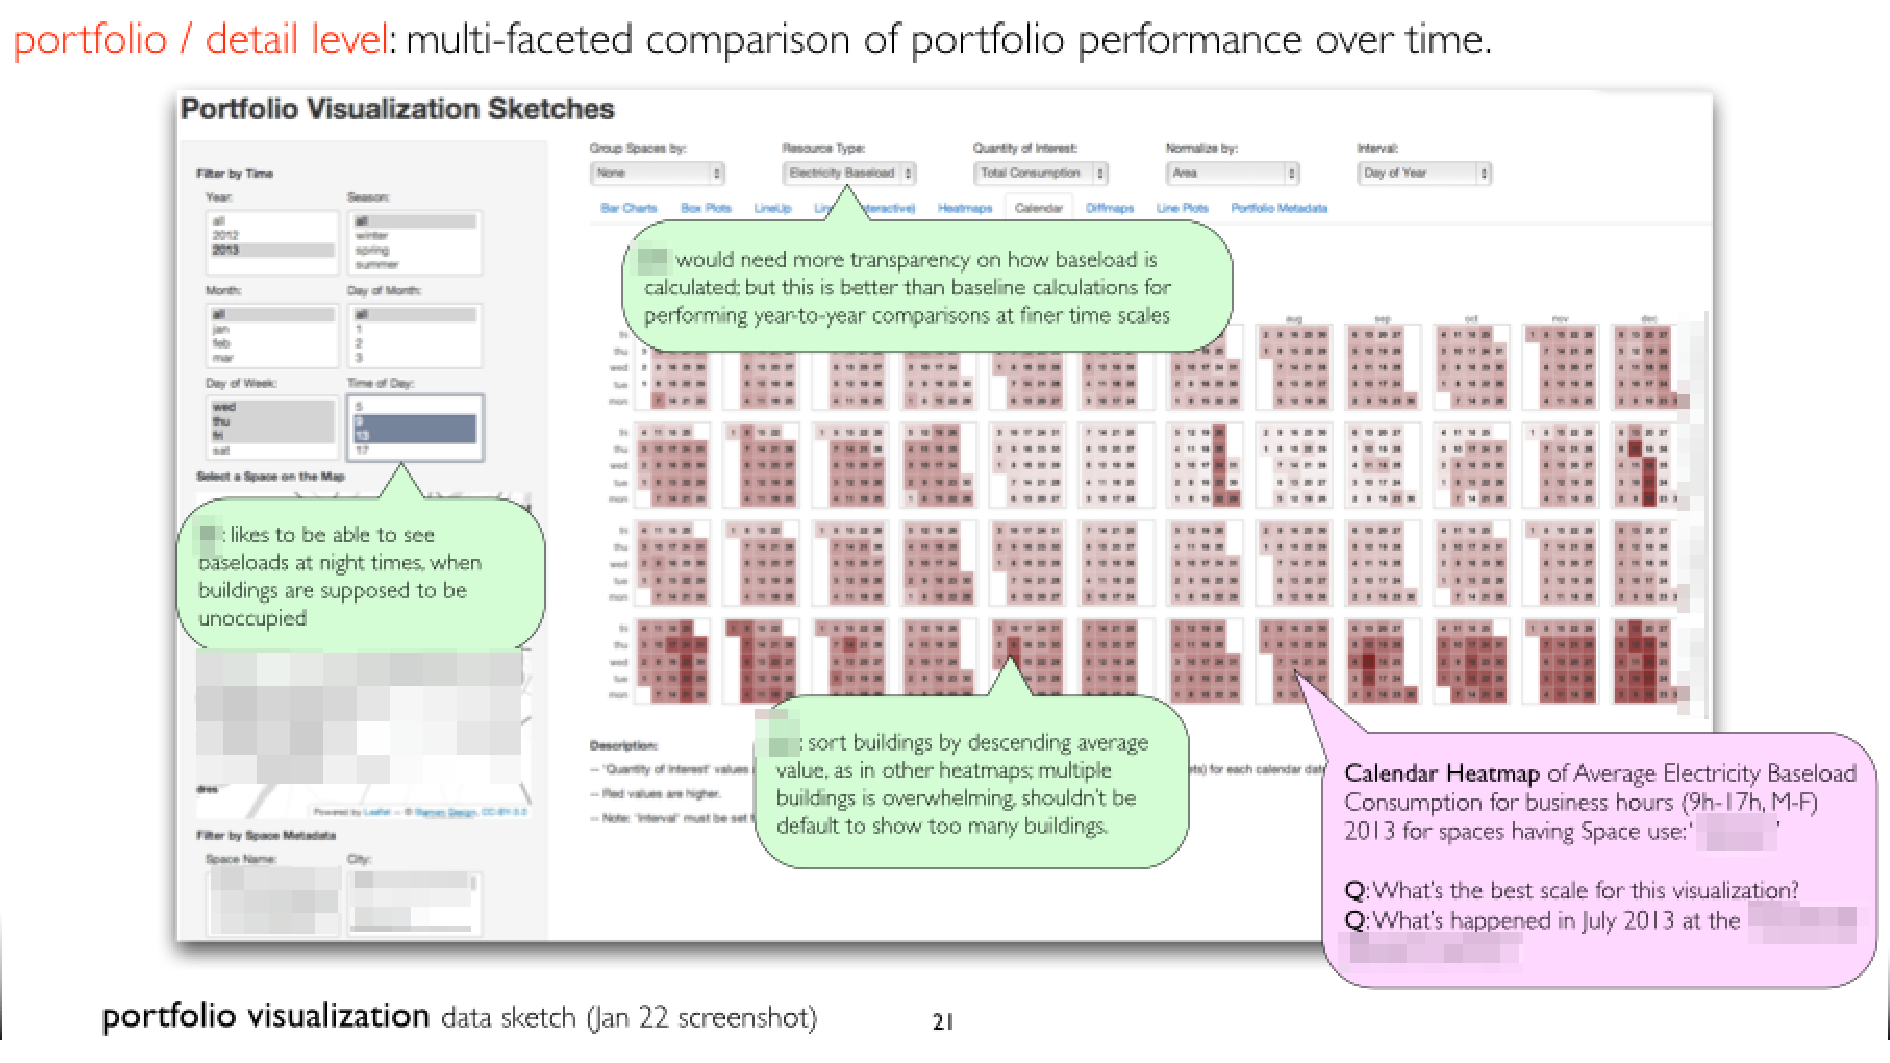
\includegraphics[width=0.975\textwidth]{figures/s-emu-08.pdf}}
	\caption
	[
	    Following-up with the power user energy analysts with designs from our sandbox design.
	]
	{
    	Following-up with the power user energy analysts with designs from our sandbox design: calendar-partitioned time series matrix (January 2014). 
	}
	\centering
	\label{app:emu:fig:follow-up}
\end{figure}

%-|-|-|-|-|-|-|-|-|-|-|-|-|-|-|-|-|-|-|-|-|-|-|-|-|-|-|-|-|-|-|-|-|-|-|-|-

%-|-|-|-|-|-|-|-|-|-|-|-|-|-|-|-|-|-|-|-|-|-|-|-|-|-|-|-|-|-|-|-|-|-|-|-|-

\begin{figure}
	\centering
	\fbox{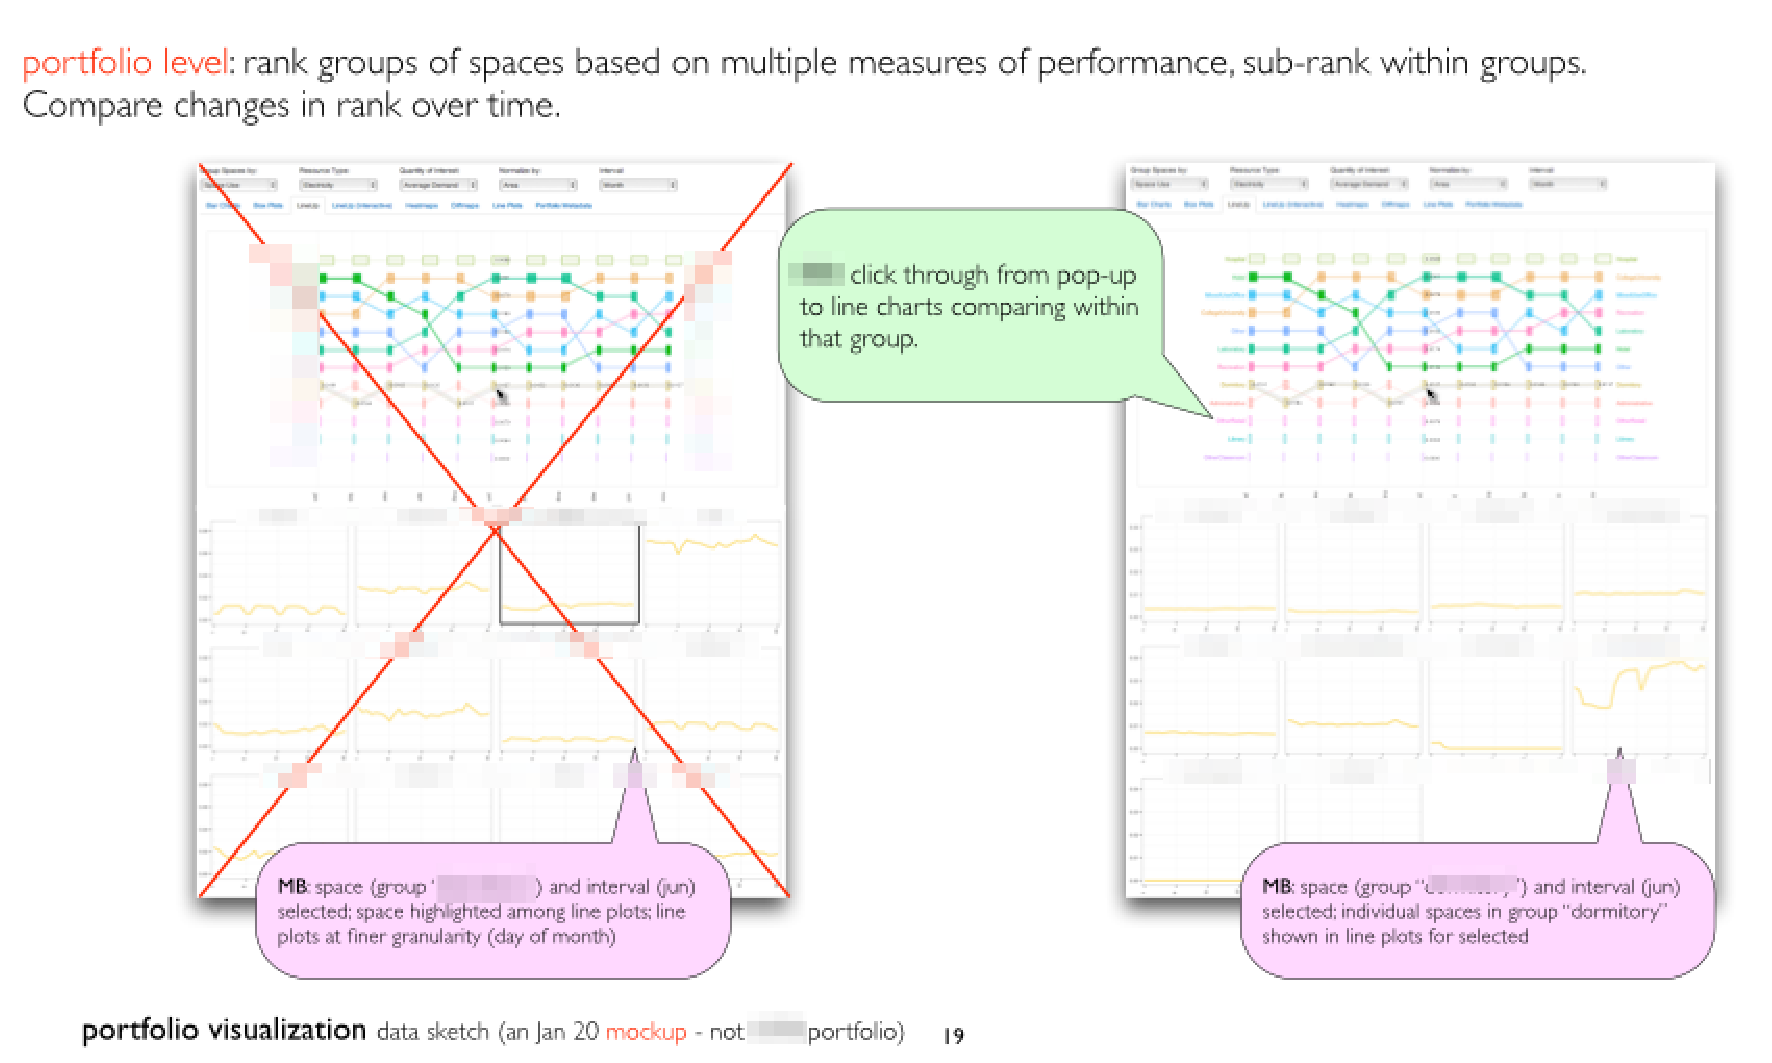
\includegraphics[width=0.975\textwidth]{figures/s-emu-08b.pdf}}
	\caption
	[
	    Following-up with the power user energy analysts with designs from our sandbox design (continued).
	]
	{
    	Following-up with the power user energy analysts with designs from our sandbox design (continued): view coordination mockups (January 2014). 
	}
	\centering
	\label{app:emu:fig:follow-up-2}
\end{figure}

%-|-|-|-|-|-|-|-|-|-|-|-|-|-|-|-|-|-|-|-|-|-|-|-|-|-|-|-|-|-|-|-|-|-|-|-|-

%-|-|-|-|-|-|-|-|-|-|-|-|-|-|-|-|-|-|-|-|-|-|-|-|-|-|-|-|-|-|-|-|-|-|-|-|-

\begin{figure}
	\centering
	\fbox{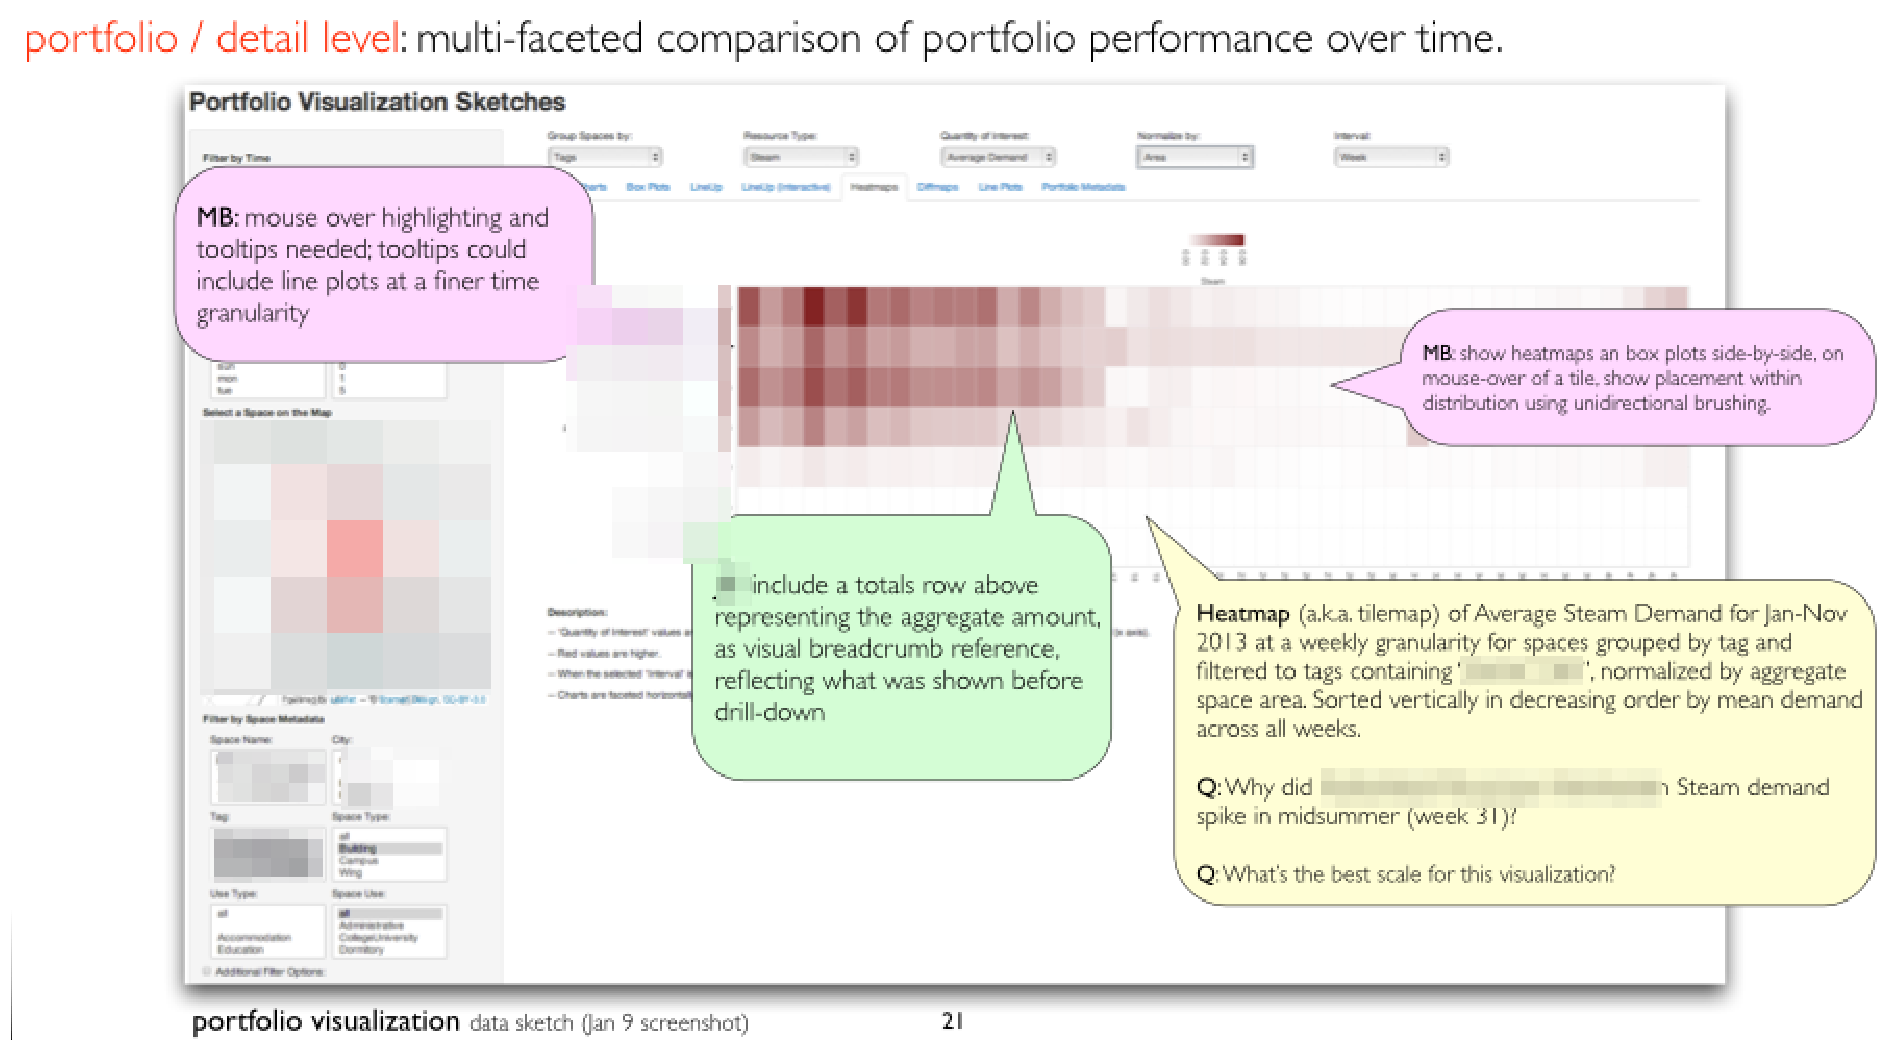
\includegraphics[width=0.975\textwidth]{figures/s-emu-10.pdf}}
	\caption
	[
	    Another iteration of data sketches produced using the sandbox environment.
	]
	{
    	Another iteration of data sketches produced using the sandbox environment: time series matrix (January 2014). 
	}
	\centering
	\label{app:emu:fig:sketches}
\end{figure}

%-|-|-|-|-|-|-|-|-|-|-|-|-|-|-|-|-|-|-|-|-|-|-|-|-|-|-|-|-|-|-|-|-|-|-|-|-

%-|-|-|-|-|-|-|-|-|-|-|-|-|-|-|-|-|-|-|-|-|-|-|-|-|-|-|-|-|-|-|-|-|-|-|-|-

\begin{figure}
	\centering
	\fbox{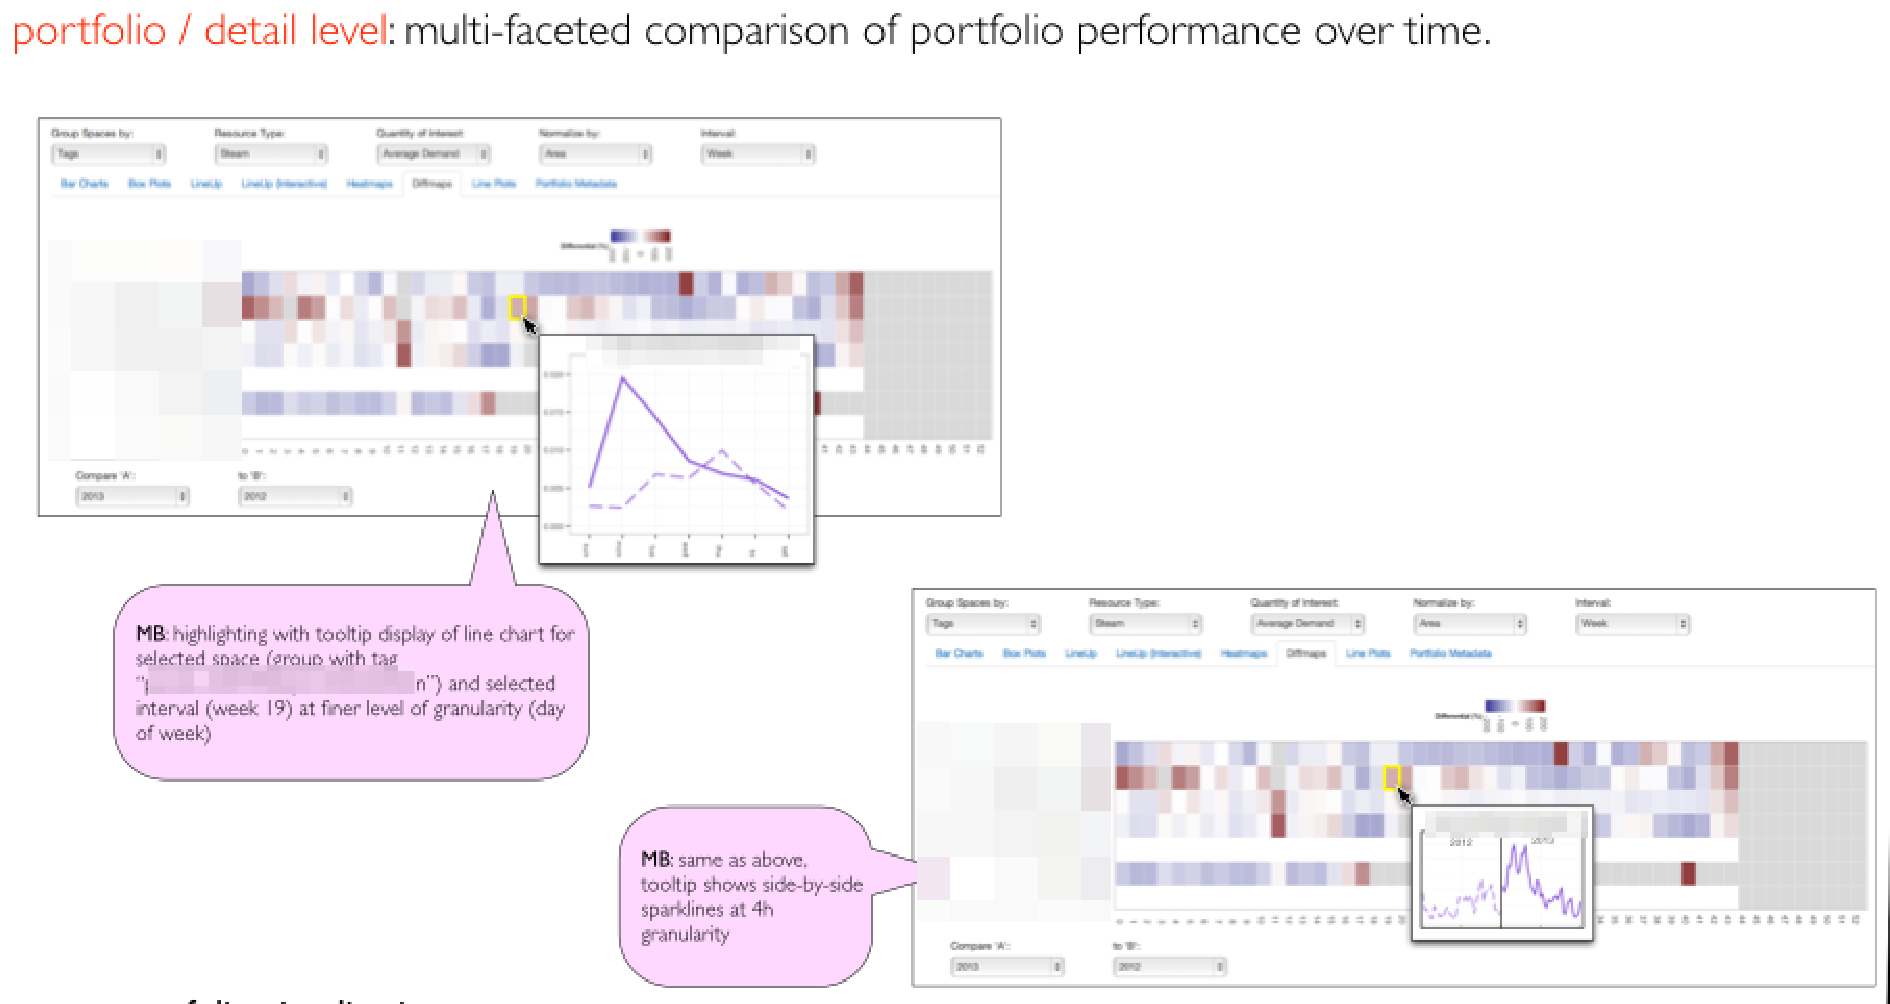
\includegraphics[width=0.975\textwidth]{figures/s-emu-10b.pdf}}
	\caption
	[
	    Another iteration of data sketches produced using the sandbox environment (continued).
	]
	{
    	Another iteration of data sketches produced using the sandbox environment (continued): interactivity mockups (January 2014). 
	}
	\centering
	\label{app:emu:fig:sketches-2}
\end{figure}

%-|-|-|-|-|-|-|-|-|-|-|-|-|-|-|-|-|-|-|-|-|-|-|-|-|-|-|-|-|-|-|-|-|-|-|-|-

%-|-|-|-|-|-|-|-|-|-|-|-|-|-|-|-|-|-|-|-|-|-|-|-|-|-|-|-|-|-|-|-|-|-|-|-|-

\begin{figure}
	\centering
	\fbox{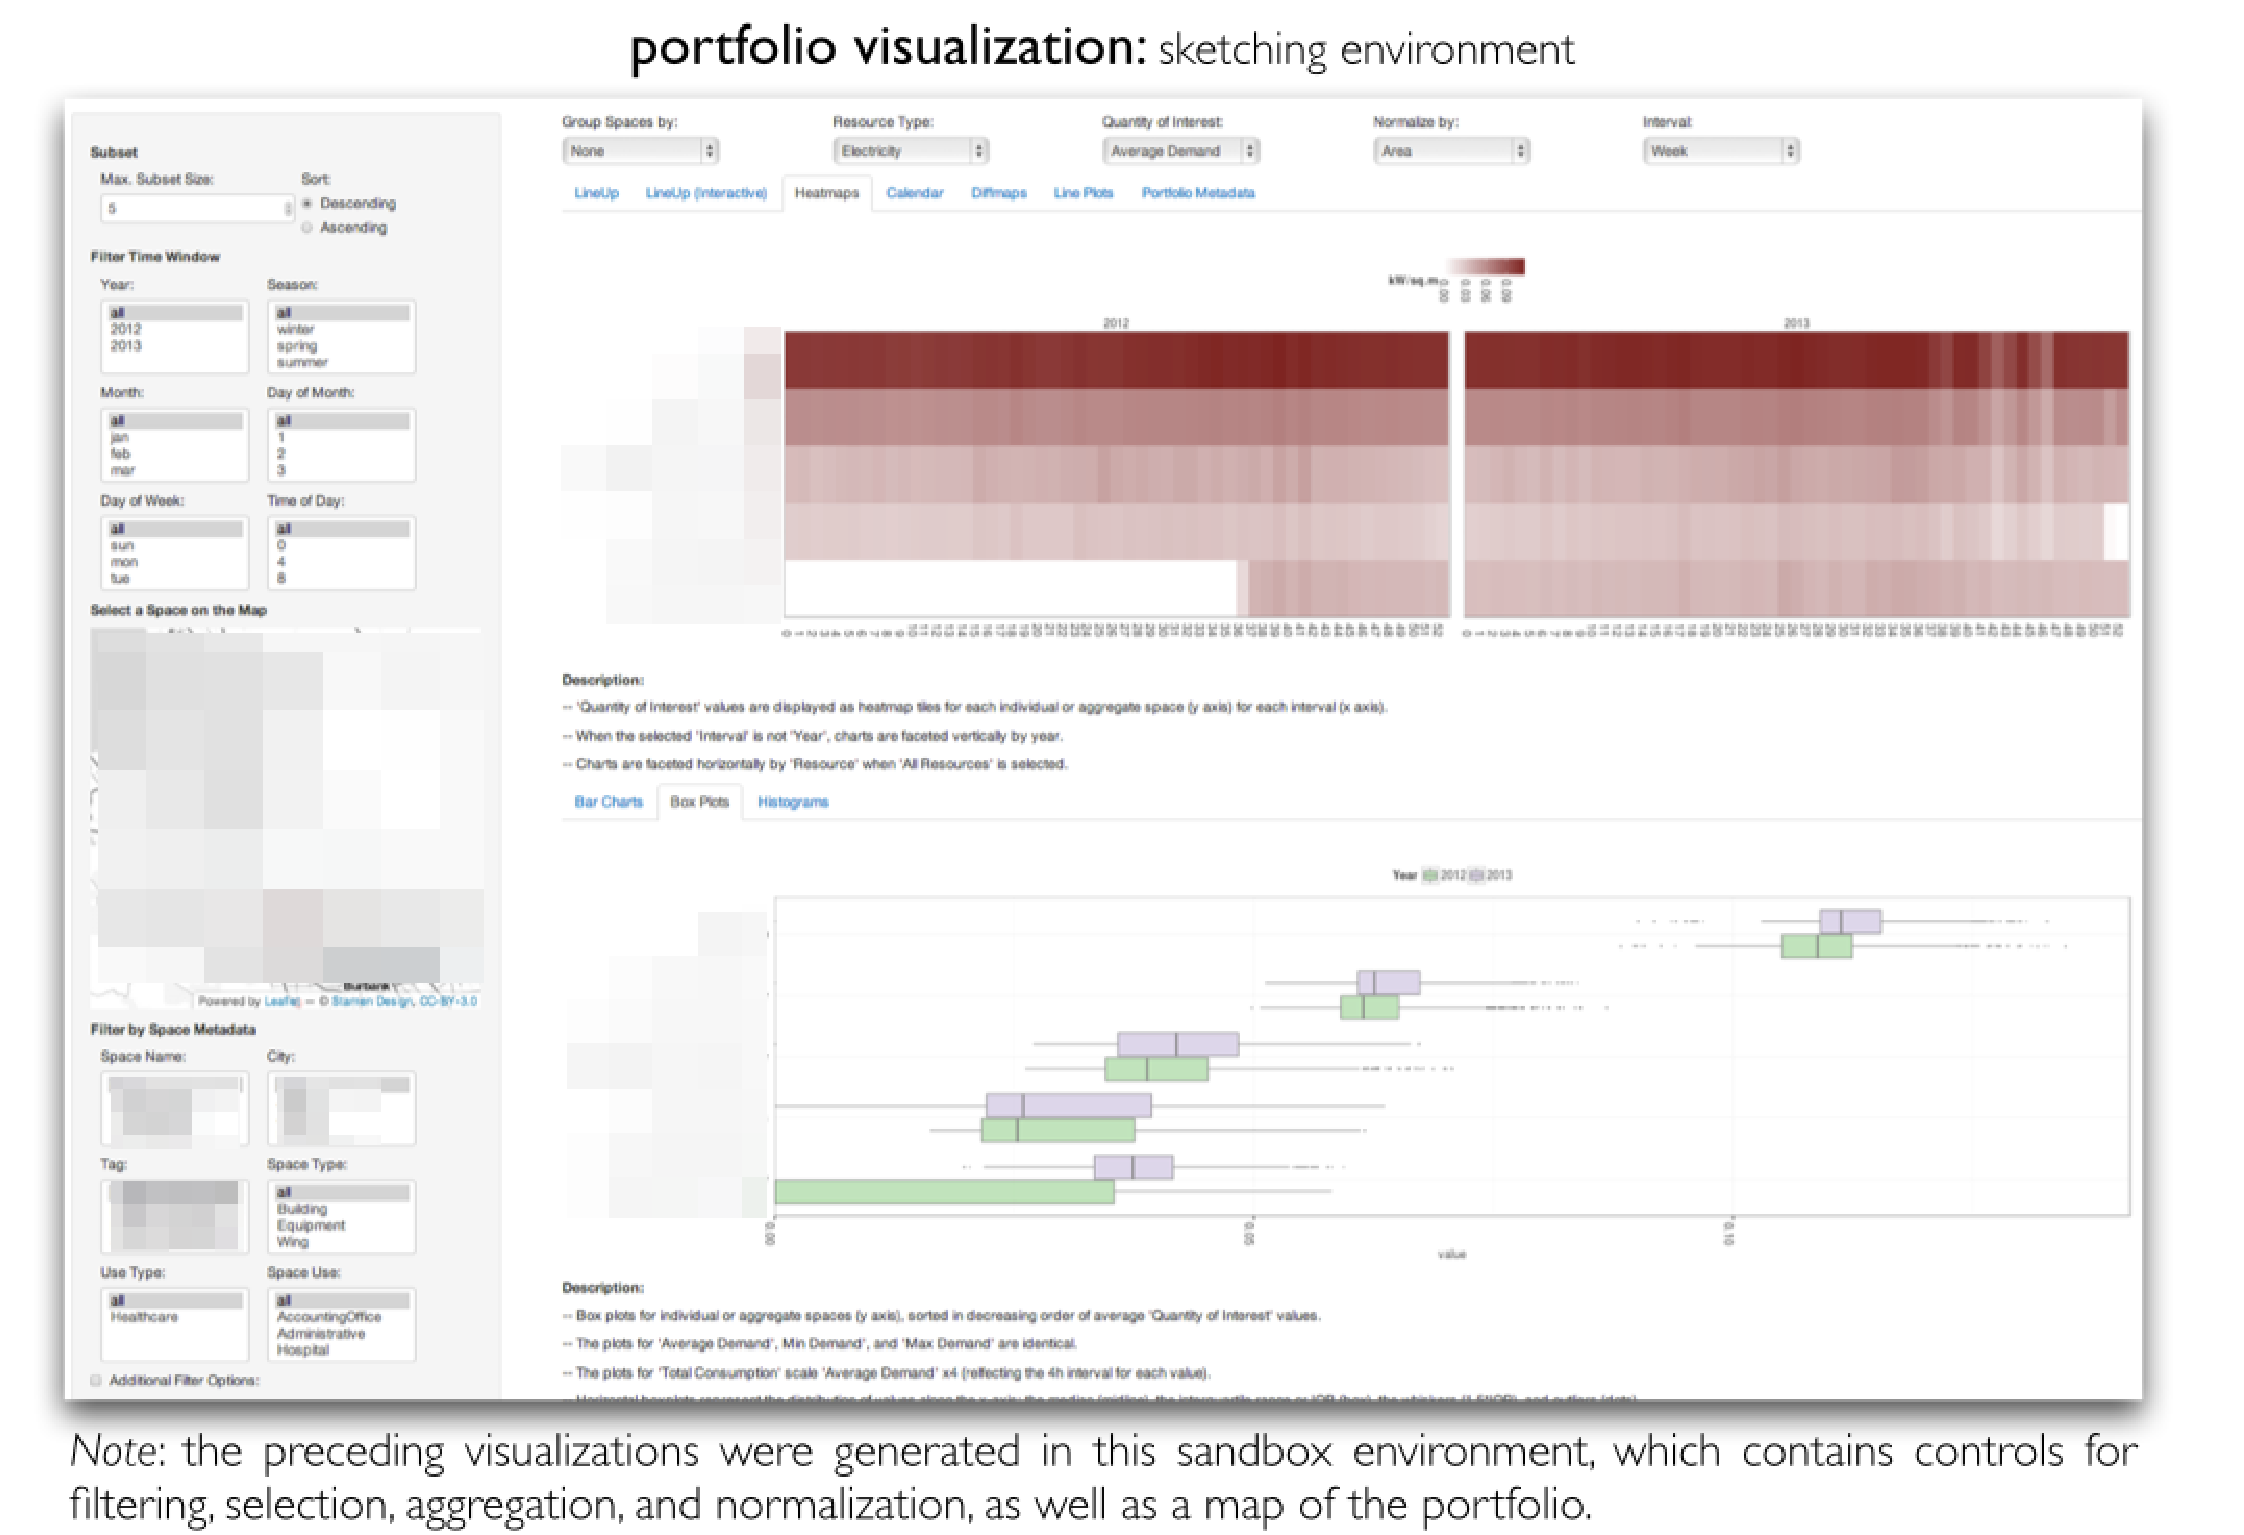
\includegraphics[width=0.975\textwidth]{figures/s-emu-09.pdf}}
	\caption
	[
	    Early view coordination design depicting a matrix with auxiliary boxplots.
	]
	{
    	Early view coordination design depicting a matrix with auxiliary boxplots (February 2014). 
	}
	\centering
	\label{app:emu:fig:boxplots}
\end{figure}

%-|-|-|-|-|-|-|-|-|-|-|-|-|-|-|-|-|-|-|-|-|-|-|-|-|-|-|-|-|-|-|-|-|-|-|-|-

%-|-|-|-|-|-|-|-|-|-|-|-|-|-|-|-|-|-|-|-|-|-|-|-|-|-|-|-|-|-|-|-|-|-|-|-|-

\begin{figure}
	\centering
	\fbox{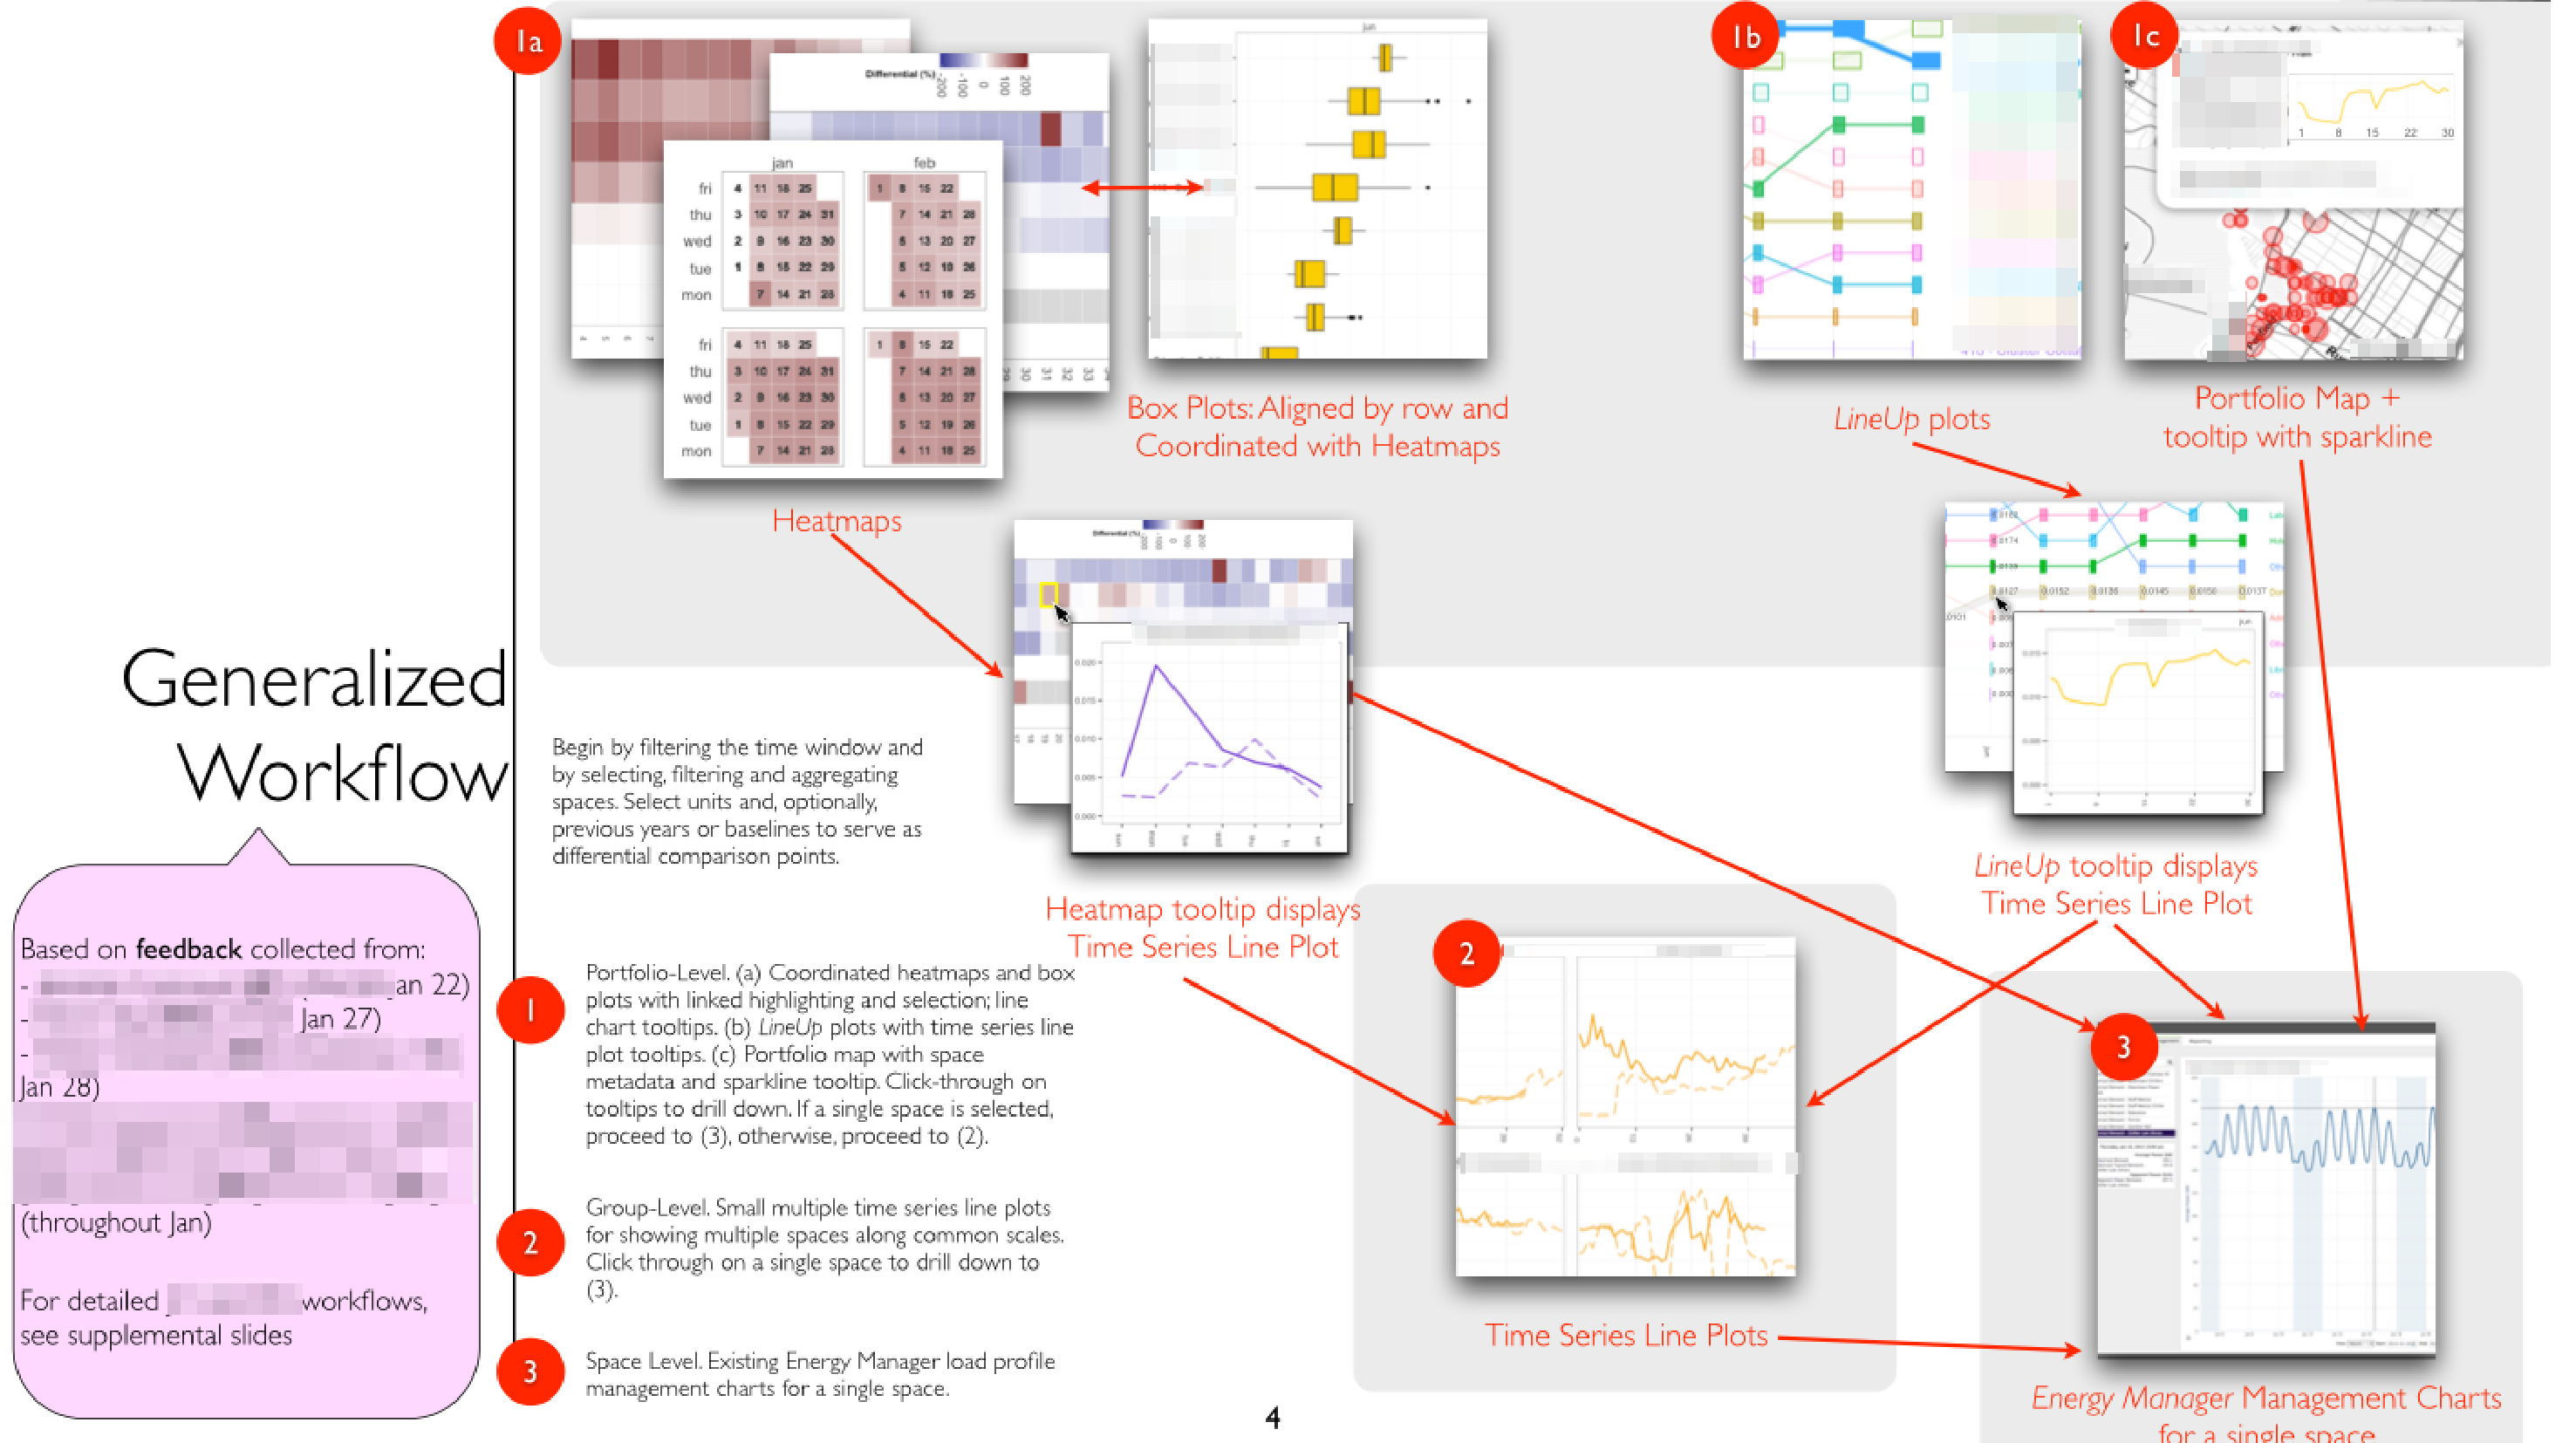
\includegraphics[width=0.975\textwidth]{figures/s-emu-11.pdf}}
	\caption
	[
	    Proposed workflow design involving multiple views based on consolidated feedback from energy analysts.
	]
	{
    	Proposed workflow design involving multiple views based on consolidated feedback from energy analysts (February 2014). 
	}
	\centering
	\label{app:emu:fig:workflow}
\end{figure}

%-|-|-|-|-|-|-|-|-|-|-|-|-|-|-|-|-|-|-|-|-|-|-|-|-|-|-|-|-|-|-|-|-|-|-|-|-

%-|-|-|-|-|-|-|-|-|-|-|-|-|-|-|-|-|-|-|-|-|-|-|-|-|-|-|-|-|-|-|-|-|-|-|-|-

\begin{figure}
	\centering
	\fbox{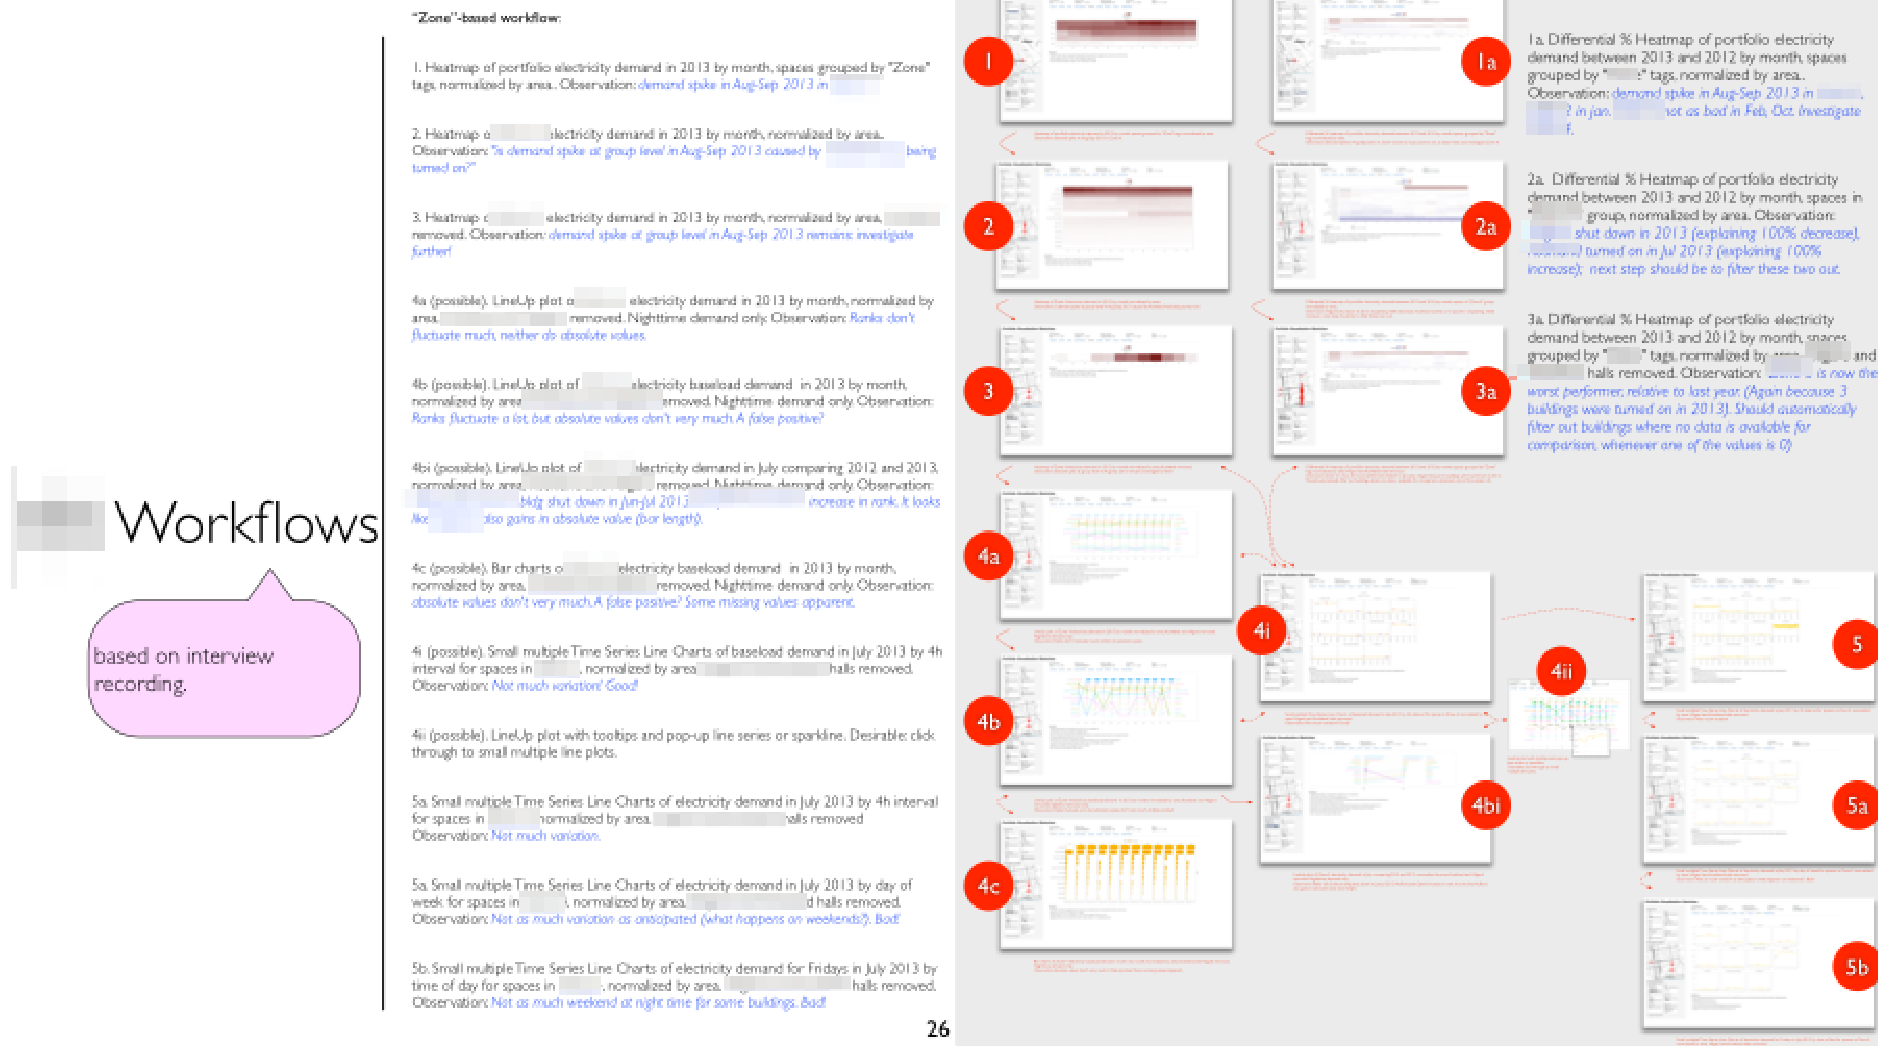
\includegraphics[width=0.975\textwidth]{figures/s-emu-12.pdf}}
	\caption
	[
	    Storyboards using sandbox screenshots based on power user workflows.
	]
	{
    	Storyboards using sandbox screenshots based on power user workflows (February 2014). 
	}
	\centering
	\label{app:emu:fig:storyboards}
\end{figure}

%-|-|-|-|-|-|-|-|-|-|-|-|-|-|-|-|-|-|-|-|-|-|-|-|-|-|-|-|-|-|-|-|-|-|-|-|-

%-|-|-|-|-|-|-|-|-|-|-|-|-|-|-|-|-|-|-|-|-|-|-|-|-|-|-|-|-|-|-|-|-|-|-|-|-

\begin{figure}
	\centering
	\fbox{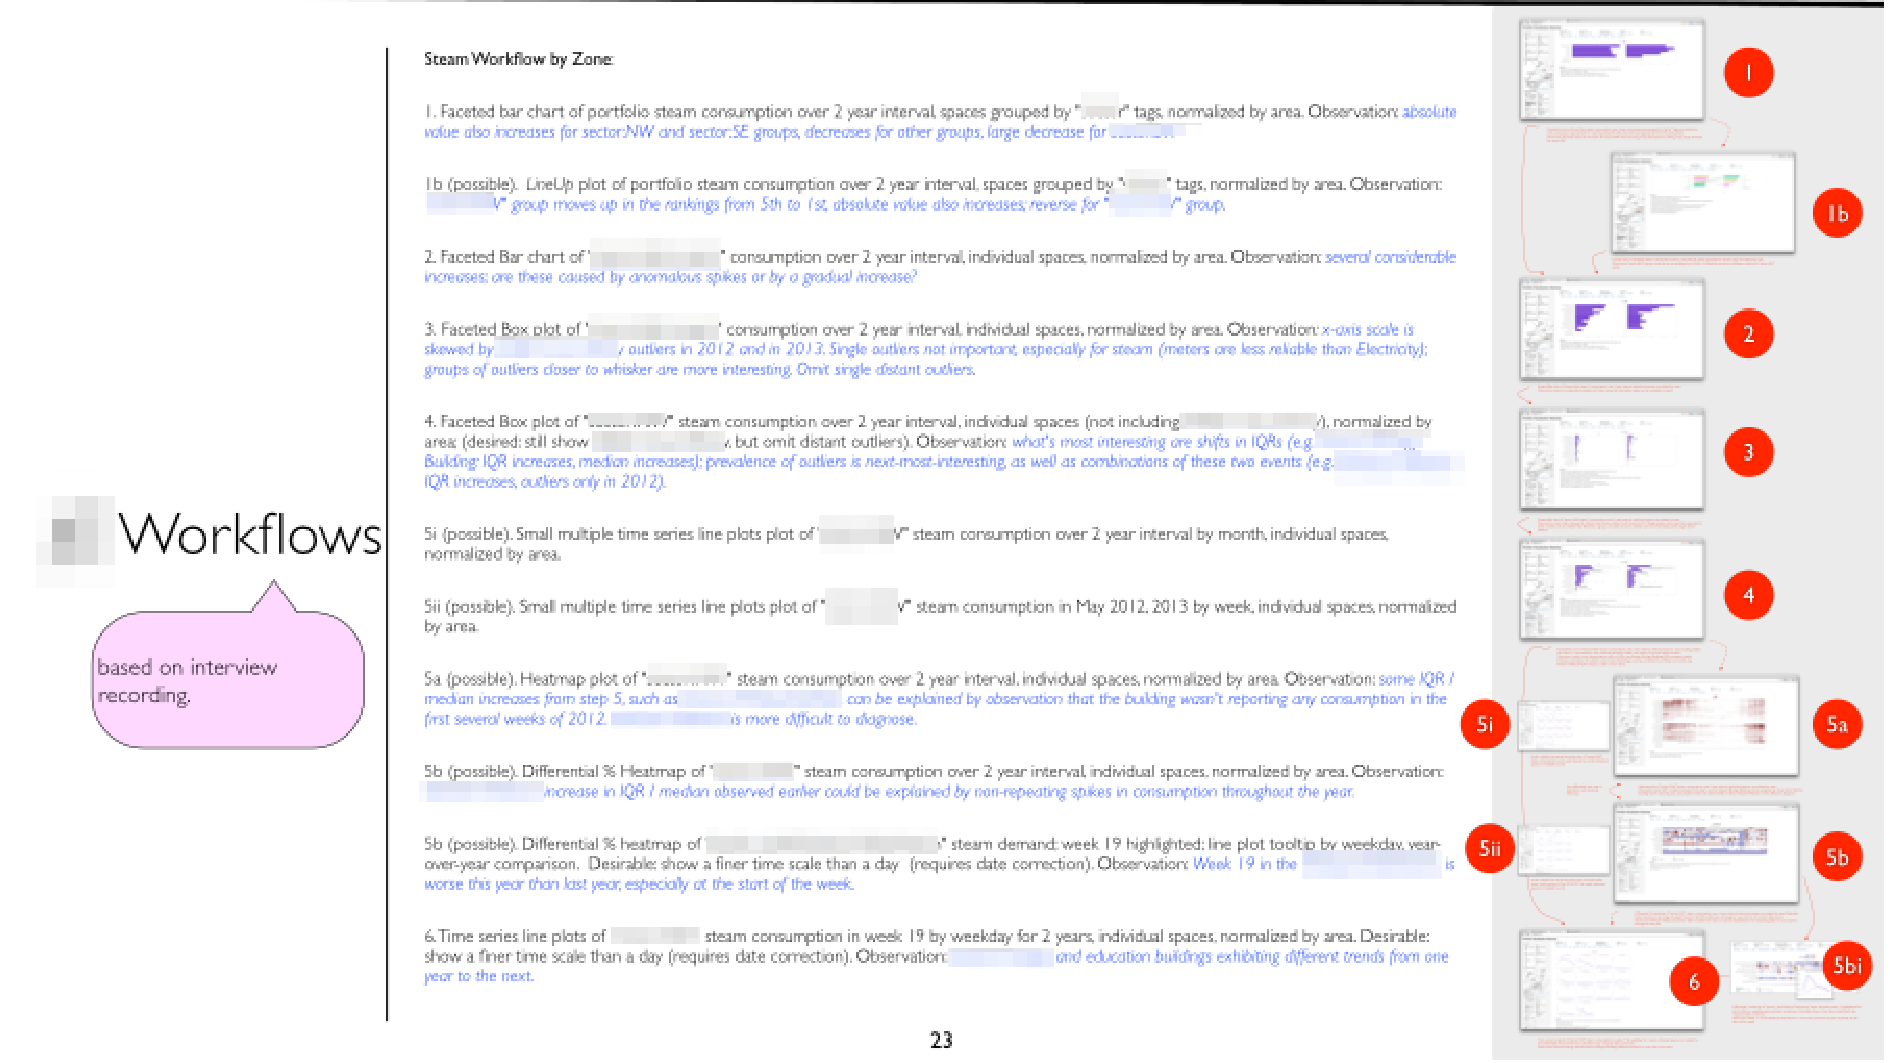
\includegraphics[width=0.975\textwidth]{figures/s-emu-12b.pdf}}
	\caption
	[
	    Storyboards using sandbox screenshots based on power user workflows (continued).
	]
	{
    	Storyboards using sandbox screenshots based on power user workflows (continued) (February 2014). 
	}
	\centering
	\label{app:emu:fig:storyboards-2}
\end{figure}

%-|-|-|-|-|-|-|-|-|-|-|-|-|-|-|-|-|-|-|-|-|-|-|-|-|-|-|-|-|-|-|-|-|-|-|-|-

\autoref{app:emu:fig:color-stock}, \autoref{app:emu:fig:brushed-boxplots}, and \autoref{app:emu:fig:juxt-boxplots} are screenshots of D3.js~\cite{Bostock2011} prototypes developed in Summer 2014 that address view coordination\index{view coordination} design.

%-|-|-|-|-|-|-|-|-|-|-|-|-|-|-|-|-|-|-|-|-|-|-|-|-|-|-|-|-|-|-|-|-|-|-|-|-

\begin{figure}
	\centering
	\fbox{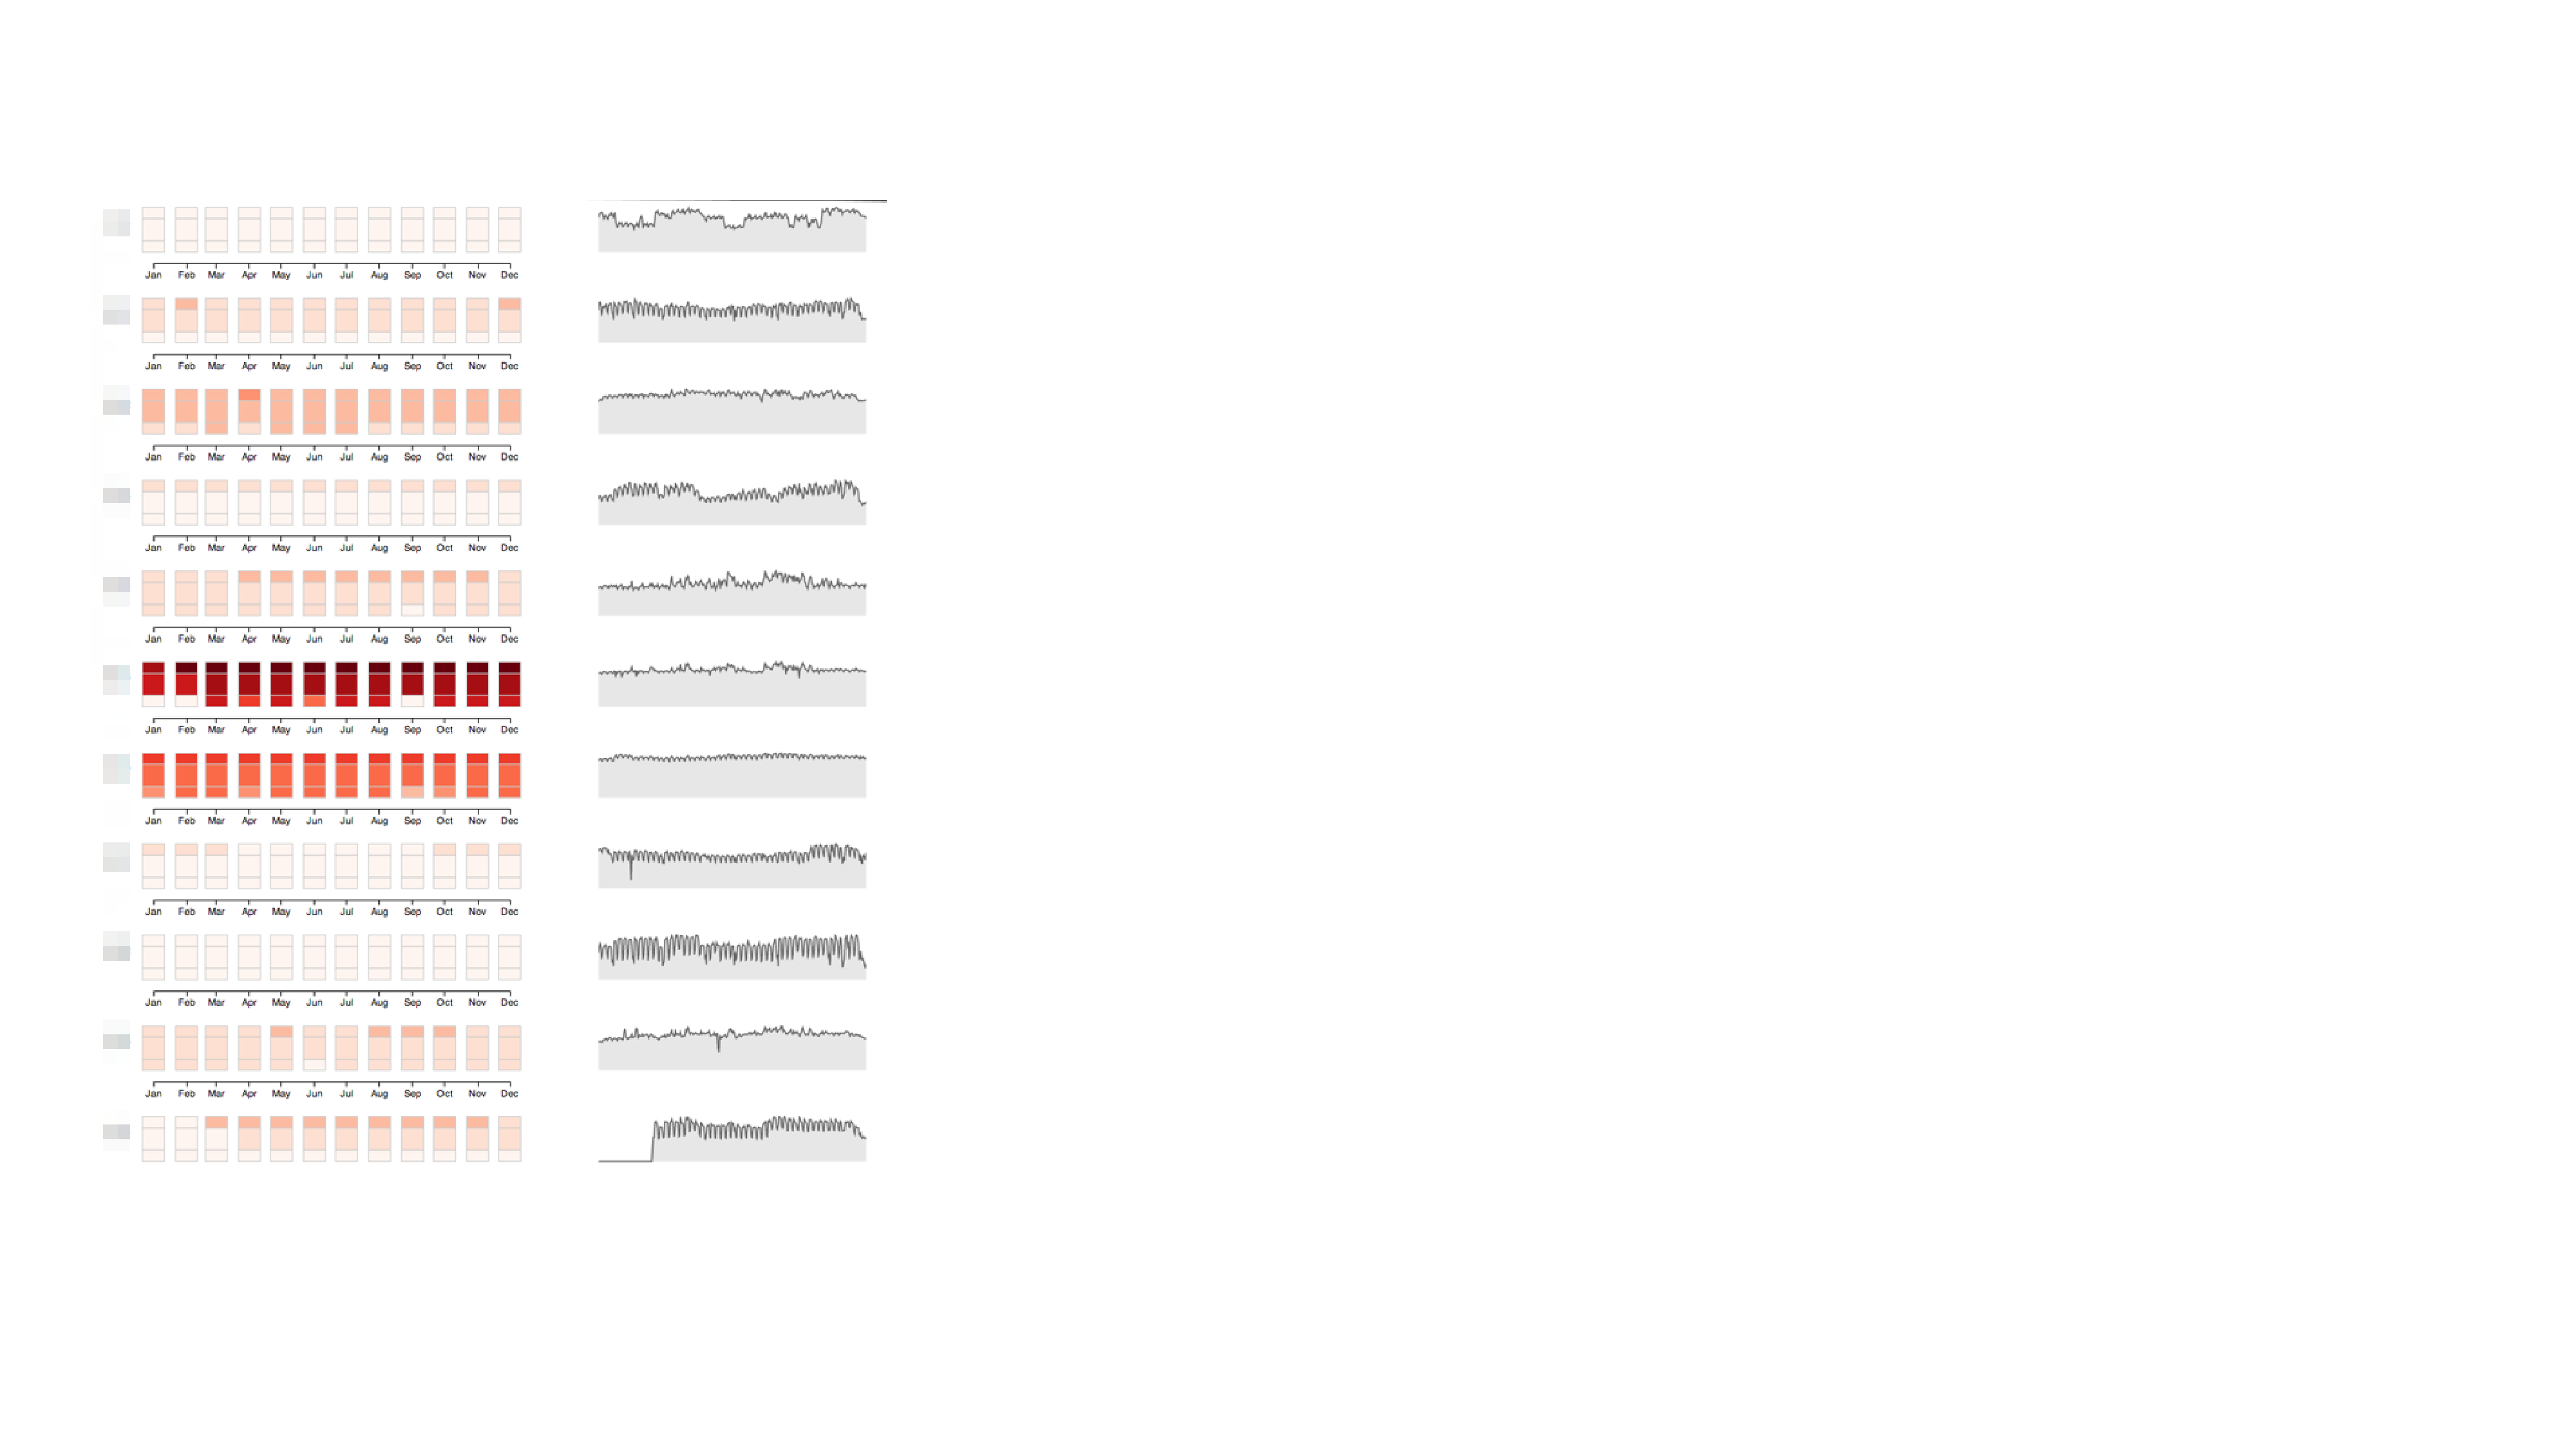
\includegraphics[width=0.975\textwidth]{figures/s-emu-13.pdf}}
	\caption
	[
	    Color stock charts with juxtaposed line charts as alternative to matrix with juxtaposed boxplots.
	]
	{
    	Color stock charts~\cite{Albers2014} with juxtaposed line charts as alternative to matrix with juxtaposed boxplots (Summer 2014). 
	}
	\centering
	\label{app:emu:fig:color-stock}
\end{figure}

%-|-|-|-|-|-|-|-|-|-|-|-|-|-|-|-|-|-|-|-|-|-|-|-|-|-|-|-|-|-|-|-|-|-|-|-|-

%-|-|-|-|-|-|-|-|-|-|-|-|-|-|-|-|-|-|-|-|-|-|-|-|-|-|-|-|-|-|-|-|-|-|-|-|-

\begin{figure}
	\centering
	\fbox{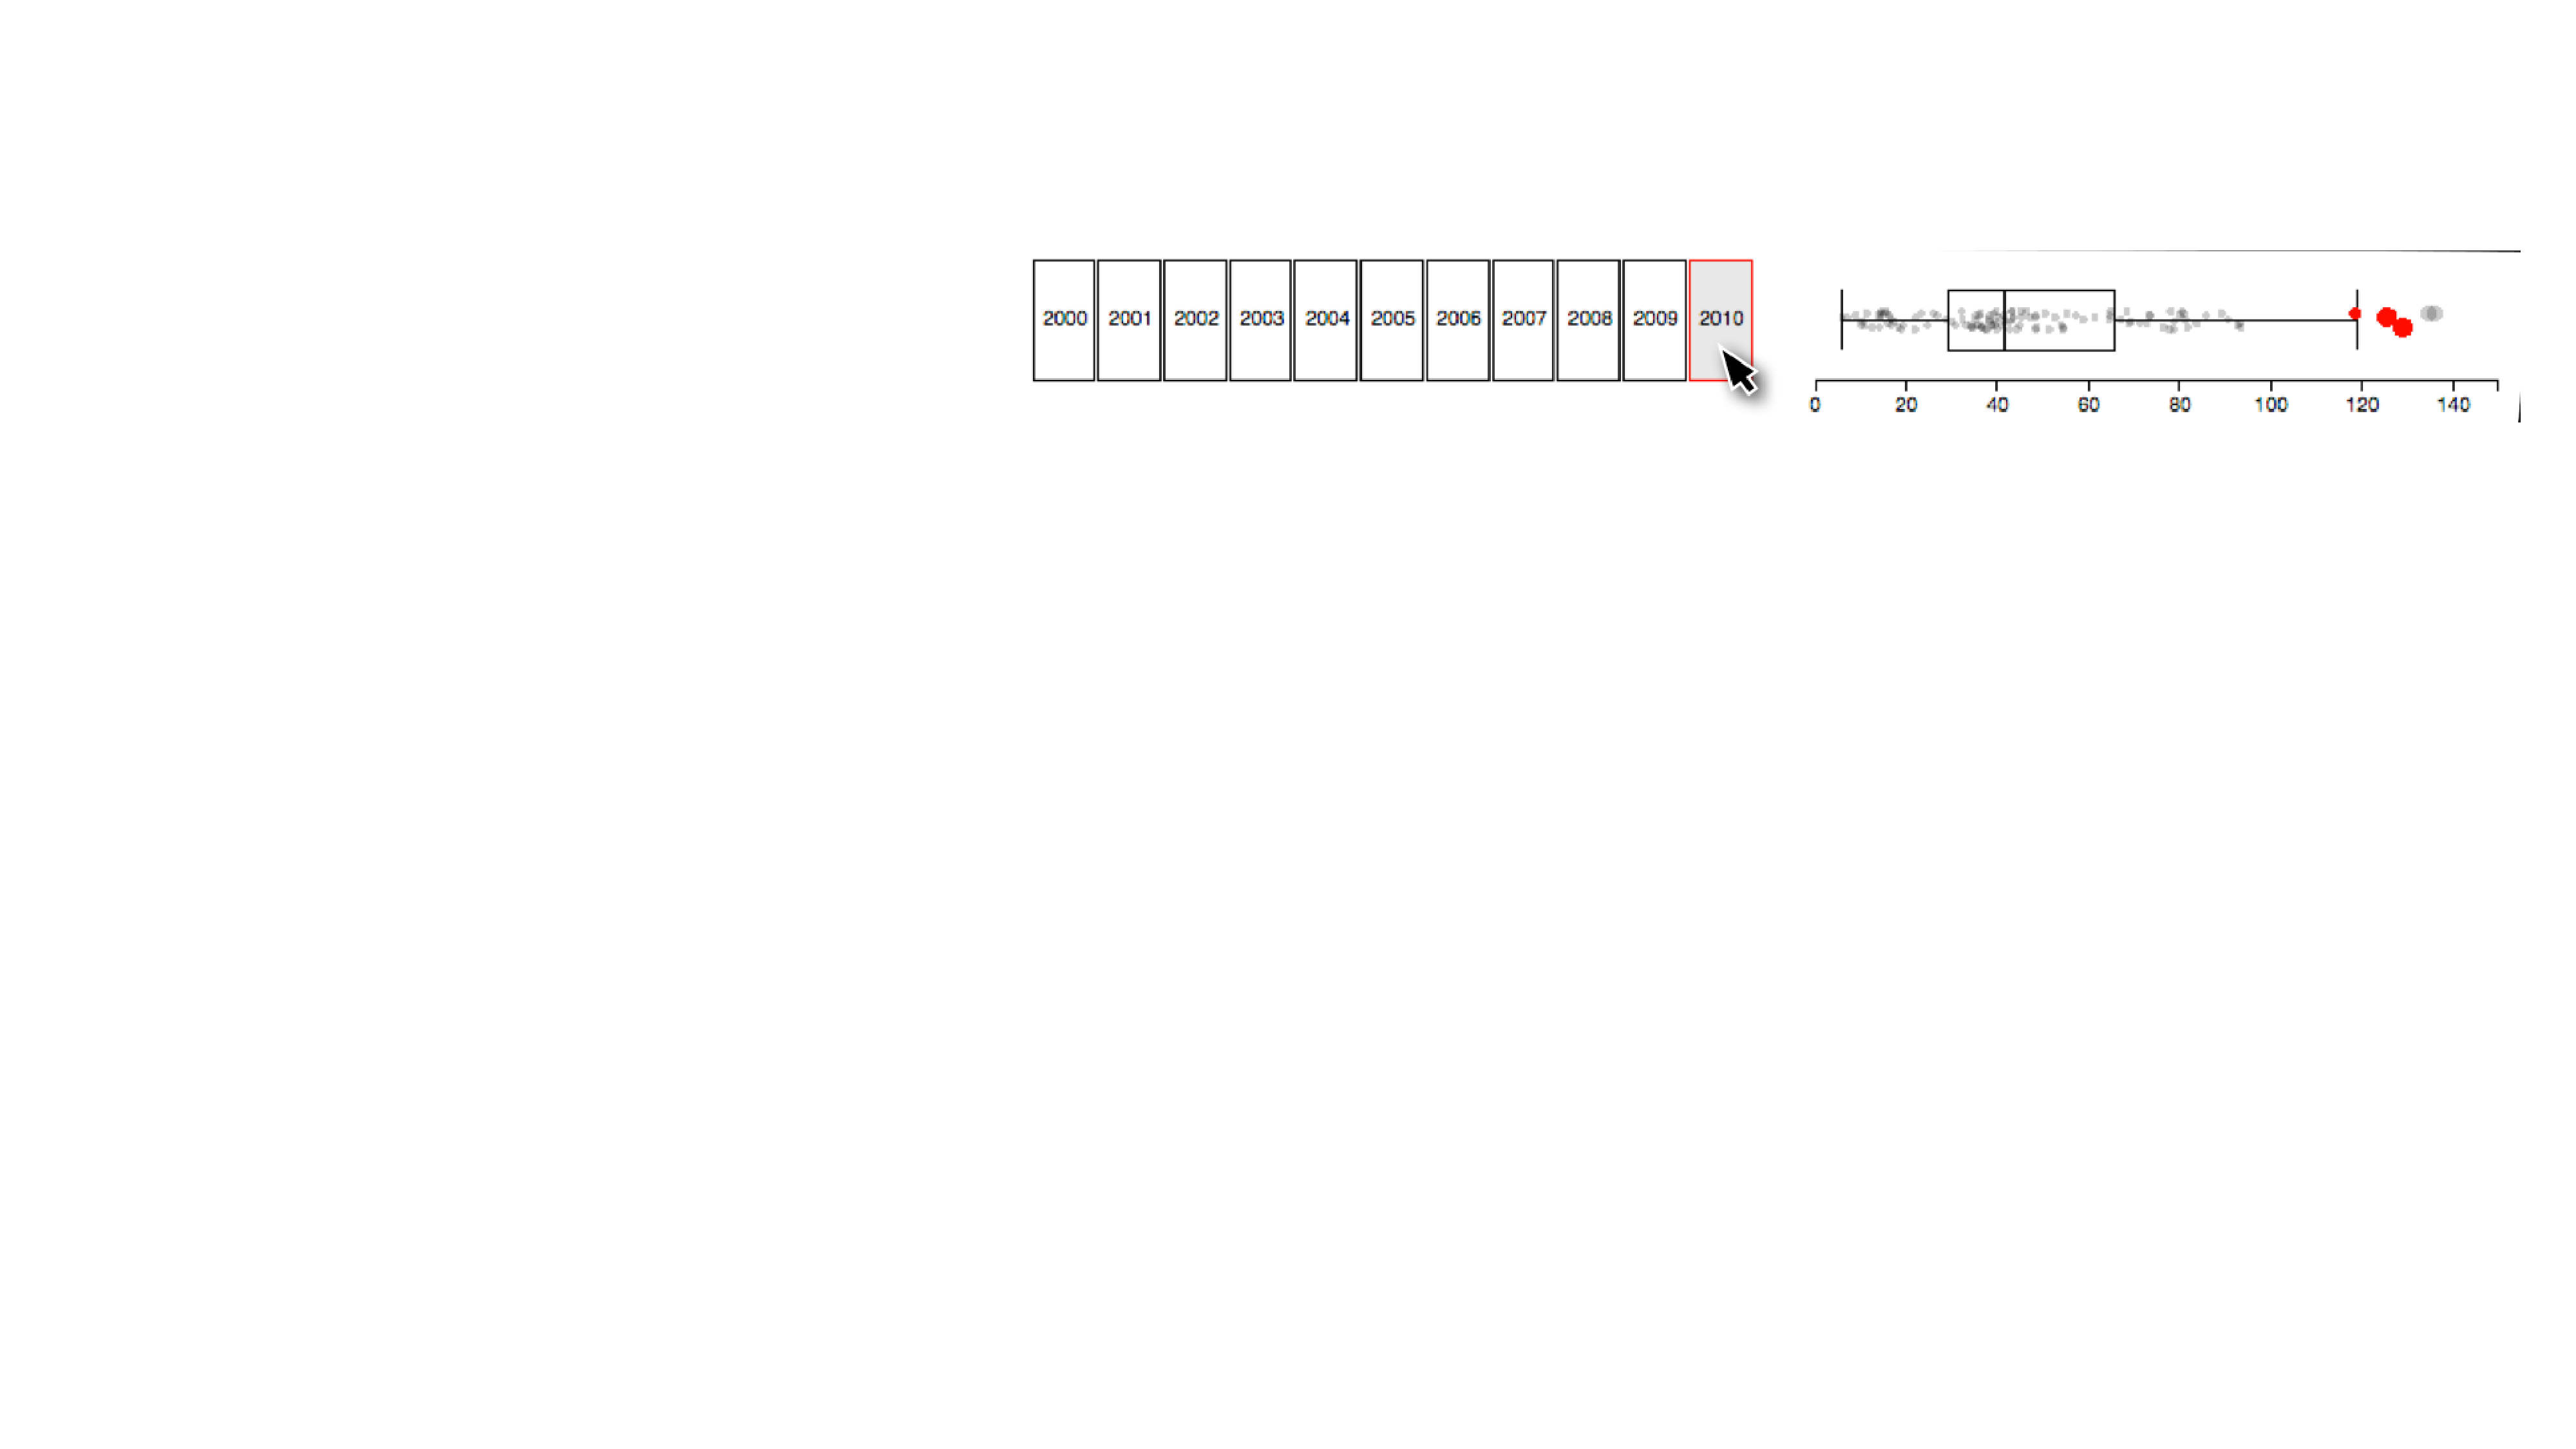
\includegraphics[width=0.975\textwidth]{figures/s-emu-14.pdf}}
	\caption
	[
	    Values from the brushed time period are highlighted on the juxtaposed boxplots.
	]
	{
    	Values from the brushed time period are highlighted on the juxtaposed boxplots (\url{http://bl.ocks.org/mattbrehmer/8be29724bdd7a63ff41d}) (Summer 2014). 
	}
	\centering
	\label{app:emu:fig:brushed-boxplots}
\end{figure}

%-|-|-|-|-|-|-|-|-|-|-|-|-|-|-|-|-|-|-|-|-|-|-|-|-|-|-|-|-|-|-|-|-|-|-|-|-

%-|-|-|-|-|-|-|-|-|-|-|-|-|-|-|-|-|-|-|-|-|-|-|-|-|-|-|-|-|-|-|-|-|-|-|-|-

\begin{figure}
	\centering
	\fbox{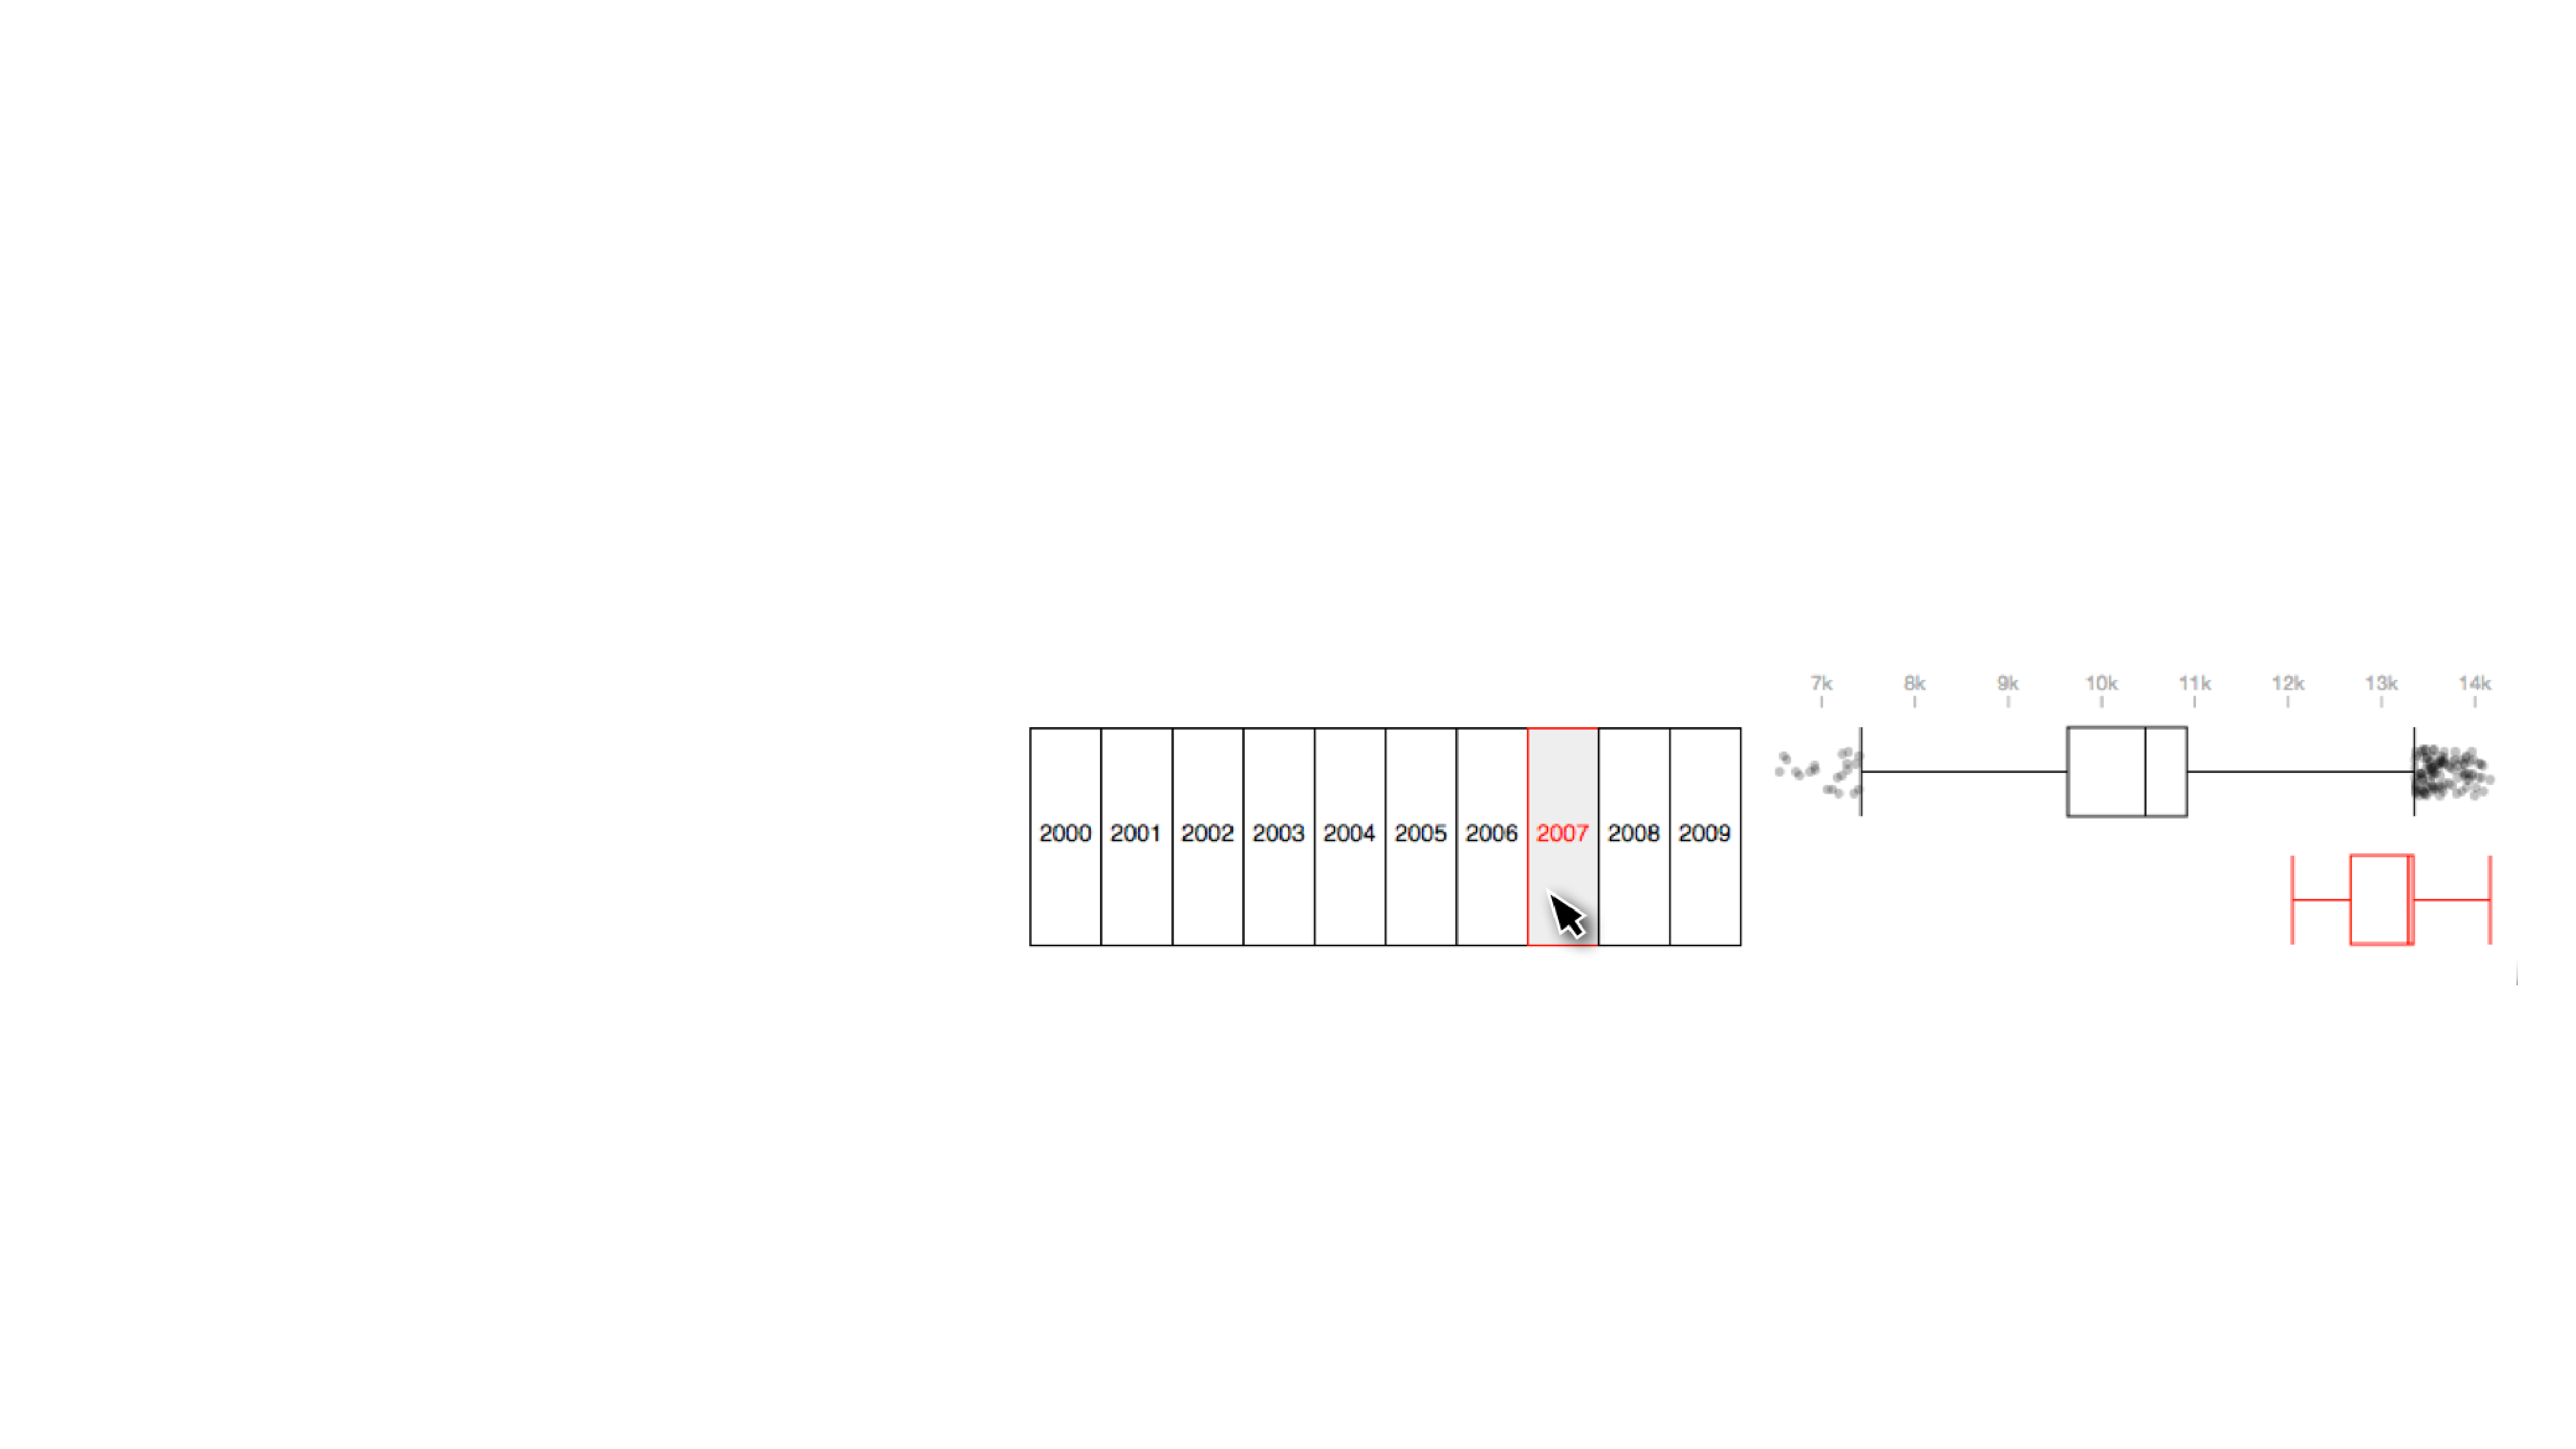
\includegraphics[width=0.975\textwidth]{figures/s-emu-15.pdf}}
	\caption
	[
	    Boxplot for the brushed time period (red) is shown alongside the boxplot for the entire time series.
	]
	{
        Boxplot for the brushed time period (red) is shown alongside the boxplot for the entire time series (\url{http://bl.ocks.org/mattbrehmer/287e44c9a12151967874}) (Summer 2014). 
	}
	\centering
	\label{app:emu:fig:juxt-boxplots}
\end{figure}

%-|-|-|-|-|-|-|-|-|-|-|-|-|-|-|-|-|-|-|-|-|-|-|-|-|-|-|-|-|-|-|-|-|-|-|-|-

Development on the redesigned Energy Manager\index{Energy Manager} continued throughout Summer 2014.
During this time, we collected feedback on the new designs from five energy analysts at EnerNOC.
\autoref{app:emu:fig:continued-feedback} provides an example of how this feedback was documented.

%-|-|-|-|-|-|-|-|-|-|-|-|-|-|-|-|-|-|-|-|-|-|-|-|-|-|-|-|-|-|-|-|-|-|-|-|-

\begin{figure}
	\centering
	\fbox{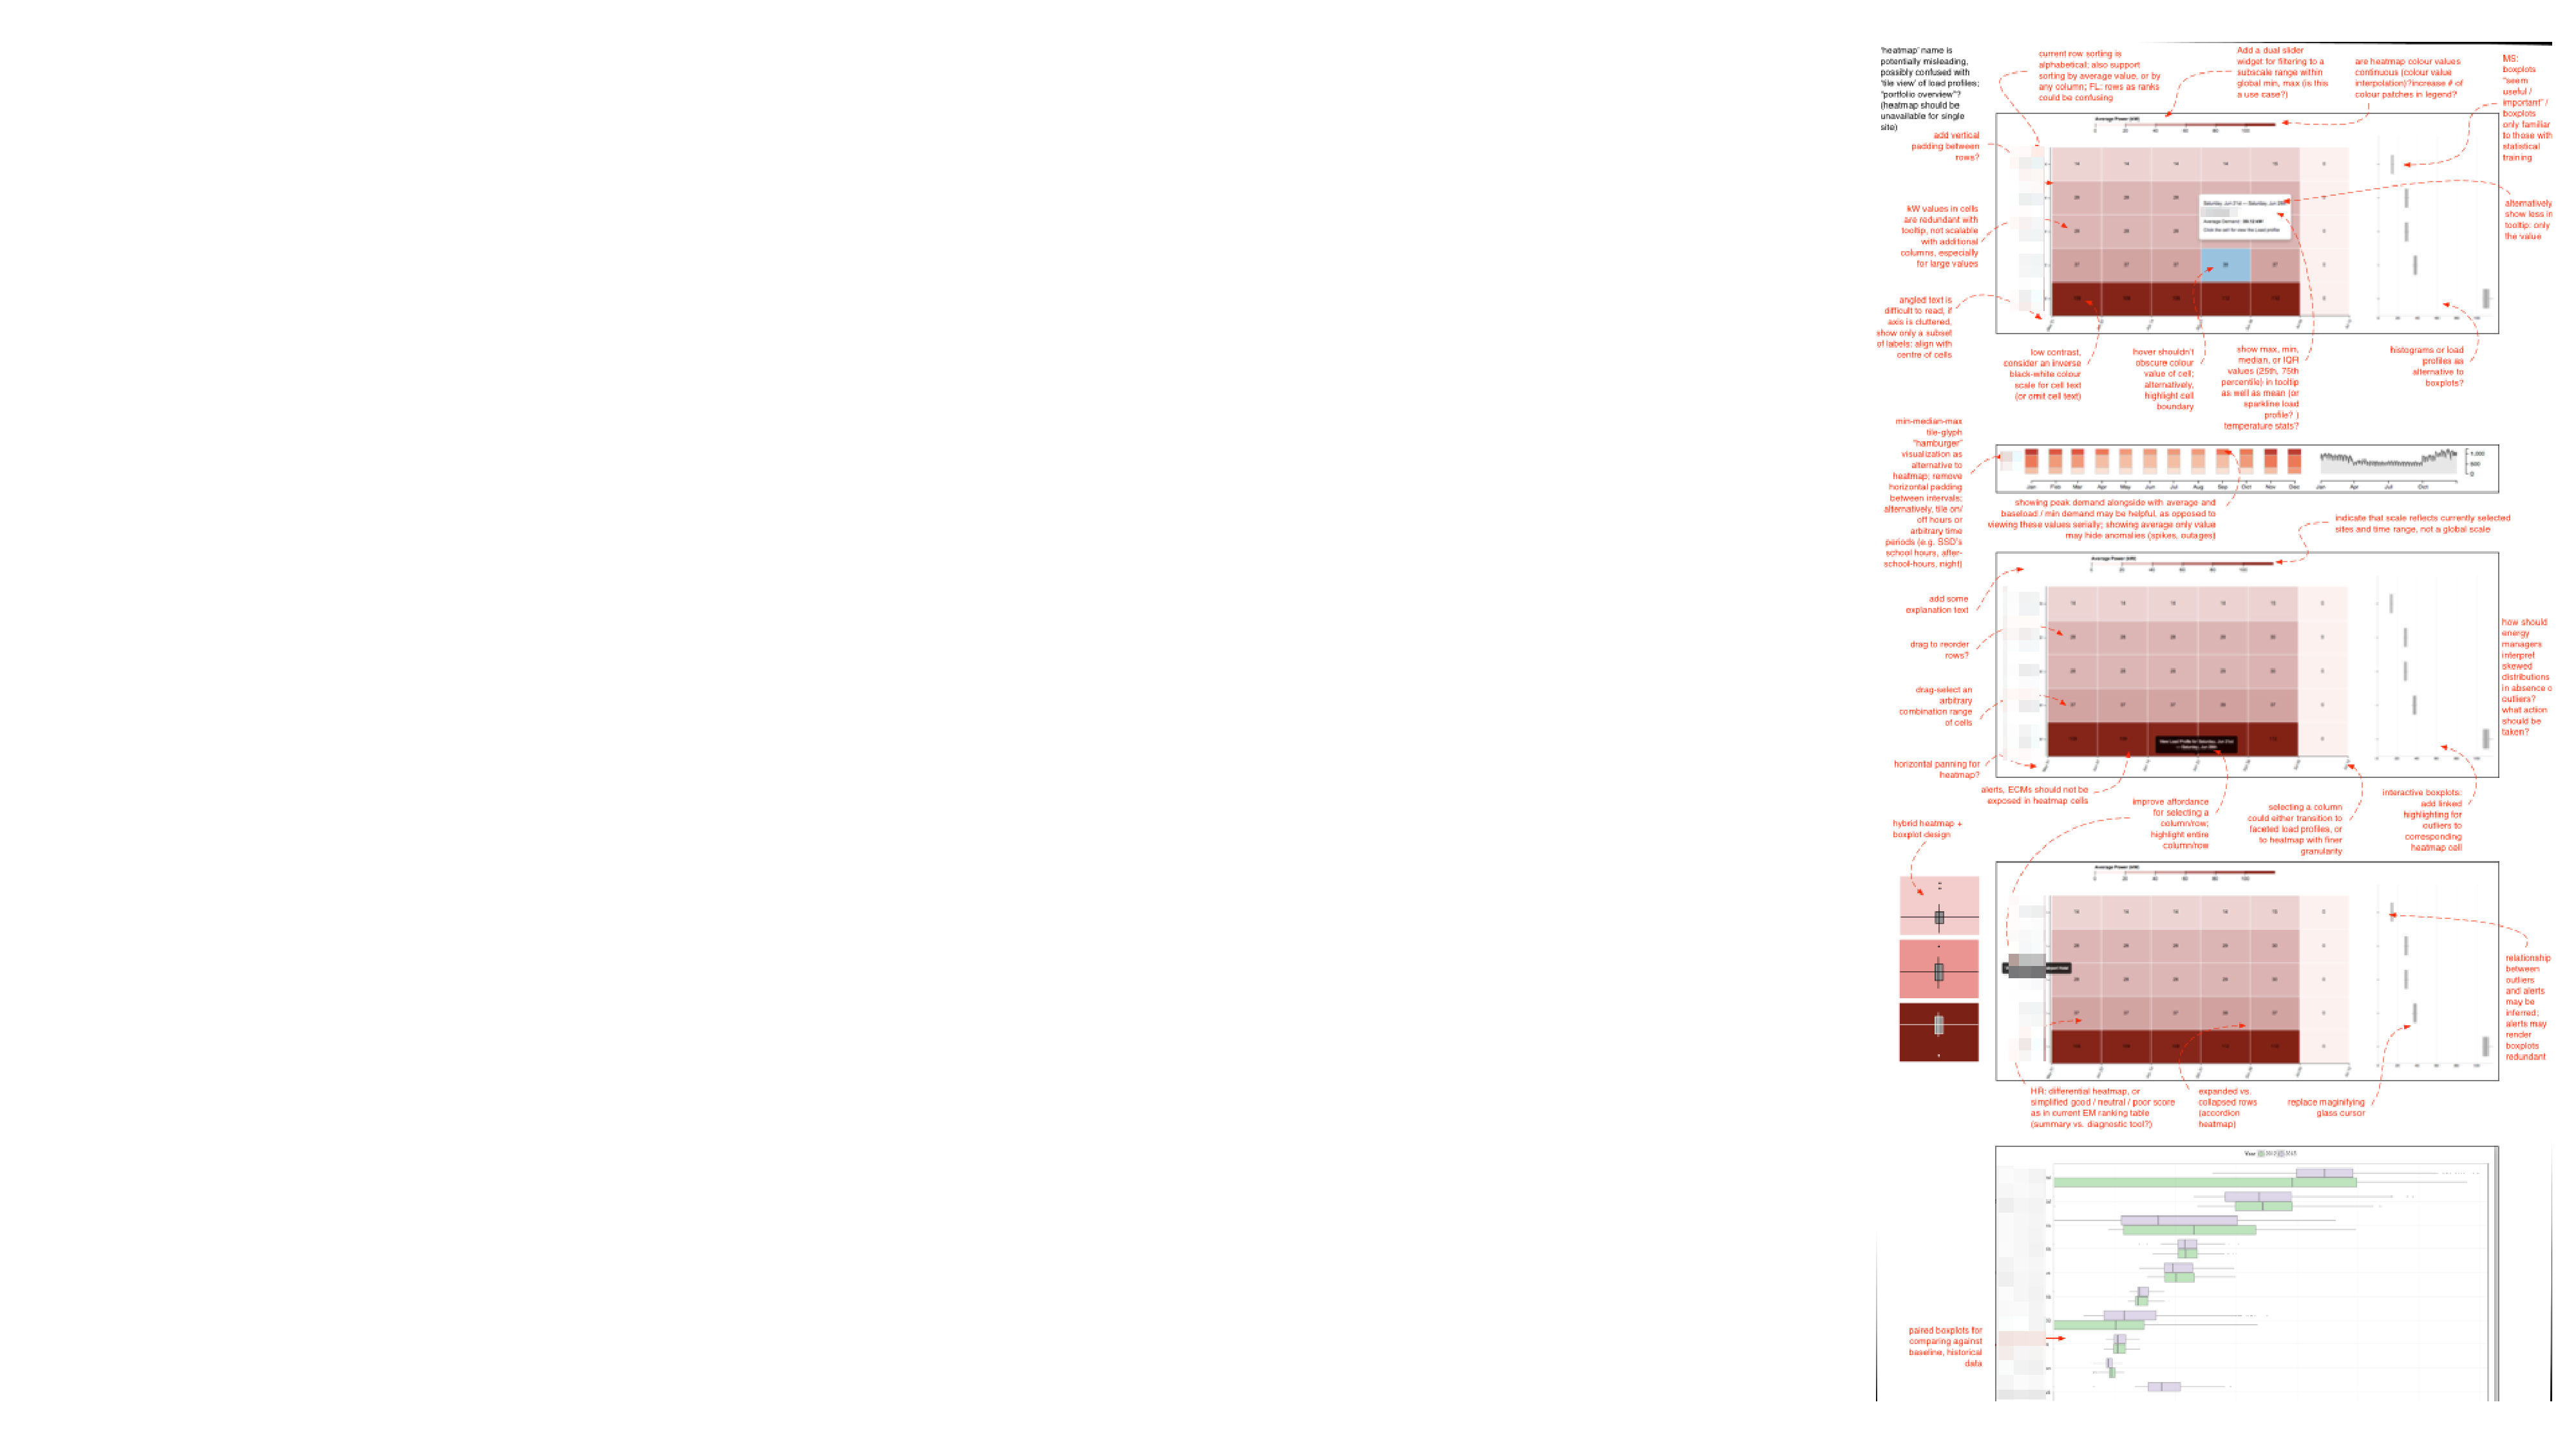
\includegraphics[width=0.65\textwidth]{figures/s-emu-16.pdf}}
	\caption
	[
	    An example of how feedback was documented.
	]
	{
        An example of how this feedback was documented, using a combination of screenshots from the redesigned Energy Manager and earlier mockups (Summer 2014). 
	}
	\centering
	\label{app:emu:fig:continued-feedback}
\end{figure}

%-|-|-|-|-|-|-|-|-|-|-|-|-|-|-|-|-|-|-|-|-|-|-|-|-|-|-|-|-|-|-|-|-|-|-|-|-